\documentclass[11pt, oneside]{article}   	% use "amsart" instead of "article" for AMSLaTeX format
\usepackage[margin = 1.1in]{geometry}            		% See geometry.pdf to learn the layout options. There are lots.
\geometry{letterpaper}                   		% ... or a4paper or a5paper or ... 
\usepackage[parfill]{parskip}    		% Activate to begin paragraphs with an empty line rather than an indent
\usepackage{graphicx}				% Use pdf, png, jpg, or eps§ with pdflatex; use eps in DVI mode
								% TeX will automatically convert eps --> pdf in pdflatex	
\usepackage{adjustbox}	
\usepackage[section]{placeins}

%% LaTeX Preamble - Common packages
\usepackage[utf8]{inputenc}
\usepackage[english]{babel}
\usepackage{textcomp} % provide lots of new symbols
\usepackage{graphicx}  % Add graphics capabilities
\usepackage{flafter}  % Don't place floats before their definition
\usepackage{amsmath,amssymb}  % Better maths support & more symbols
\usepackage[backend=biber]{biblatex}
\usepackage{amsthm}
\usepackage{bm}  % Define \bm{} to use bold math fontsx
\usepackage[pdftex,bookmarks,colorlinks,breaklinks]{hyperref}  % PDF hyperlinks, with coloured links
\usepackage{memhfixc}  % remove conflict between the memoir class & hyperref
\usepackage{mathtools}
\usepackage[T1]{fontenc}
\usepackage[scaled]{beramono}
\usepackage{listings}
\usepackage{physics}
\usepackage{tensor}
\usepackage{tikz}
\usepackage{pgfplots} 

\usepackage{helvet}

%% Commands for typesetting theorems, claims and other things. 
\newtheorem{theorem}{Theorem}
\newtheorem*{thm}{Theorem}
\newtheorem*{claim}{Claim}
\newtheorem*{example}{Example}
\newtheorem*{defn}{Definition}

\newcommand{\Lagr}{\mathcal{L}}
\newcommand{\vc}[1]{\mathbf{#1}}
\newcommand{\pdrv}[2]{\frac{\partial{#1}}{\partial{#2}}}
\newcommand{\thrint}[1]{\int d^3 \vc{x} \left( {#1} \right)}
\newcommand{\ve}[1]{ \mathbf{#1} } 
\newcommand{\spint}{ \int d^d x \, } 
\newcommand{\pdif}[2] { \frac{ \partial #1 }{ \partial #2 } } 
\newcommand{ \R}{ \mathbb{ R} } 

\title{Part III Statistical Field Theory}
\author{Notes taken by Afiq Hatta, based on Part III lectures by Matthew McCullough}
\begin{document}
\maketitle
\tableofcontents

\pagebreak 

\section{Useful resources}
\begin{itemize}
	\item David Tong's notes on statistical field theory 
	\item MIT opencourseware's lecture notes on statistical mechanics. 
\end{itemize}

\section{Introduction}

Statistical field theory studies systems with large degrees of freedom, their different 'phases'  and the transition between these phases. Think 'more is different'. When we have a large number of degrees of freedom, we can see discontinuous phenomena emerge. 

\section{Why Statistical Field Theory?} 
\subsection{Phase transitions and critical exponents} 
This set of notes will revolve around explaining the phenomena of phase transitions. In physics so far, we've described systems in terms of smooth and differentiable functions. For example, smooth paths given by solving the Euler-Lagrange equations for $N$ particles. However, in reality, many physical systems exhibit discontinuous behaviour. The most obvious of these would be a phase transition from liquid to gas, say. Or, for example, thje change in magnetisation for a system from an ordered state to a disordered state. One may ask, how can systems comprised of smooth dynamics exhibit discontinuous behaviour? 

\begin{figure}[h]
	\centering
	\includegraphics[scale=0.1]{Liquid_helium_Rollin_film.jpg}
	\caption{Helium in a 'superfluid' phase}
\end{figure}

These discontinuities appear as a result of taking an $N \rightarrow \infty$ limit for the number of particles, and our previous functions which are smooth begin to get 'squashed' into a discontinuous shape. We'll study this behaviour throughout these set of notes. The discontinuities of phase transitions occur at special values of descriptors of our physical system (for example temperature, magnetisation, pressure), which we call \textbf{critical points}. How a system behaves near critical points give rise to critical exponents. For example, the mean-field theory prediction of how magnetisation varies as $T$ reaches it's critical temperature is \[ 
m \sim (T - T_c)^\alpha,\quad \alpha = \frac{ 1}{2} \] 
where $\alpha$ is a critical exponent in this case. Or, somewhat conversely, we have another critical exponent derived from how magnetisation changes due to a change the applied magnetic field $B$, which again mean-field theory predicts to have the relationship \[ m \sim B^{ \frac{ 1}{3}} \] and in this case $\frac{ 1}{ 3}$ is another example of a critical exponent appearing in nature. 
Other quantities we might want to examine the behaviour of as we approach critical points in different variables are 
\begin{itemize} 
	\item heat capacity per unit volume, often denoted $c$, changing with as $T \rightarrow T_c $
	\item magnetic susceptibility, which is how the magentisation of a system changes in response to an ambient magentic field: \[ \chi = \frac{ \partial m}{ \partial B } \] and how this quantity also varies as temperature approaches the critical temp $T \rightarrow T_c$
	\item how density of particles, $\nu_{ \text{ gas} / \text{liquid}}$ changes when either pressure or temperature approaches a critical point 
	\item compressibility and more! 
\end{itemize}  
 
\subsection{Universality} 
A striking experimental observation that we notice with regards to critical exponents is that they seem to match for different systems despite wildly different structures. An example is the critical exponent for the magnetic susceptibility of a material $\chi$ as $T \rightarrow T_c$ and the compressiblity of a gas also as $T \rightarrow T_c$. I'll include more examples later. 

\subsection{Explaining universality with the renormalization group flow} 
The key to understanding why universality occurs is by looking at how physics changes depending on what scale we're looking at it with. This is the essensce of the renormalisation group. We'd expect a system to exhibit different physical characteristics depending if we were looking at it from the perspective of a towering giant, or the perspective of a miniscule ant.  

We provide a toy example here. Suppose that we have a grid of 16 equally spaced atoms on a grid shown in the figure below. 
\begin{figure}[!h] 
	\centering 
\begin{tikzpicture}[scale=0.5]
	\foreach \x in {0, ..., 7} 
	\foreach \y in {0, ..., 7} 
	{ 
		\fill (\x, \y) circle (2pt); 
	}  
\end{tikzpicture}
	\caption{Just atoms neatly arranged in a lattice} 
	\label{fig:atomLattice}  
\end{figure} 
Now, take your favourite physical model of some phenomoena. For example, we could take the Ising model which treats the atoms as either spin up or spin down, giving us the Hamiltonian as the primary descriptor of the system: 
\[ H(T, J ) =  - J \sum_{ \langle ij \rangle } s_i s_j  - B \sum_i s_i \] 
where we've summed over neighbouring states, and have fixed temperature $T$ as well as a coupling constant $J$, in our model. The $s_i$ denote our spin state at each location in this lattice. 

Now, having to look at every atom in this lattice is a bit difficult when fjust because of the sheer number of them. Something we could do is to group atoms which are close together, and assign something like an average composite spin at each site. One obvious way to do this is to group them up in groups of say $4$ in squares. 

\begin{figure}[!h] 
	\centering 
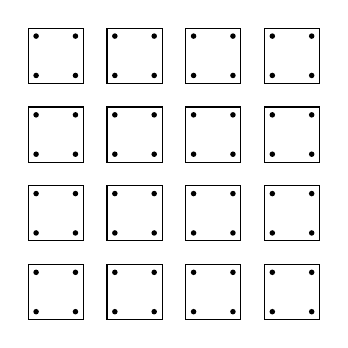
\begin{tikzpicture}[scale=0.5]
	\foreach \x in {0, ..., 7} 
	\foreach \y in {0, ..., 7} 
	{ 
		\fill (\x, \y) circle (2pt); 
	}
	\foreach \x in {0,..., 3}
	\foreach \y in {0,..., 3}  
	{ 
	\node [draw, thin, shape=rectangle, minimum width=0.7cm, minimum height=0.7cm, anchor=center] at (0.5 + 2 * \x, 0.5 + 2 * \y) {};
	}  
\end{tikzpicture}
	\qquad
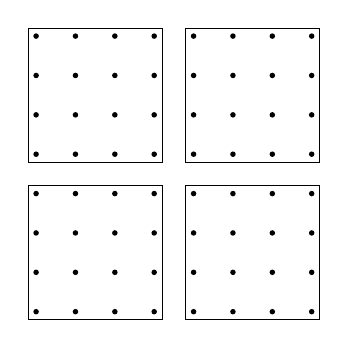
\begin{tikzpicture}[scale=0.5]
	\foreach \x in {0, ..., 7} 
	\foreach \y in {0, ..., 7} 
	{ 
		\fill (\x, \y) circle (2pt); 
	}
	\foreach \x in {0, 1} 
	\foreach \y in {0, 1} 
	{ 
			\node [draw, thin, shape=rectangle, minimum width=1.7cm, minimum height=1.7cm, anchor=center] at (1.5 + 4 * \x, 1.5 + 4 * \y) {};
	} 	  
\end{tikzpicture}
	
\caption{We can group up atoms to deal with less variables} 
	\label{fig:renormToy}  
\end{figure} 

This is shown in the first diagram. We've grouped atoms into sets of four, then we assign a single amalgamated value (like a spin average) to each group. Now, if this system exhibits \textbf{self similarity}, this means that in the new model, our structure of the Hamiltonian is the same, but our new parameters need to be changed to account for the grouping. So, our system is rewritten as \[ 
	H(J', B') = - J' \sum_{ \langle ij \rangle } \bar{s}_i \bar{s}_j  -  B' \sum_i \bar{ s}_i \]
So, by 'zooming' out of our system, we've mapped our pair of variables for from $(J, B) \rightarrow (J', B') $. This is the study of the renormalistion group. It explains universality because it predicts that different physical descriptors are just 'zoomed out' manifestations of other descriptors.  

Now, we can repeat this process even more and zoom out further, which will change the system even more. 
\subsubsection{Fixed points} 
Now, one may ask, what if we 'zoom out' according to procedures like the above, and observe the same behaviour. This is what is known as a fixed point. For example, if we had a magnetic system which is based on $T$, the temperature, and a coupling constant $J$, then if we take $T \rightarrow \infty, J = 0$, then we'll always see the same behavour of disorder no matter how much we zoom out. We'll touch on this in the later sections.

 
\section{The Ising Model and Critical Exponents}
\subsection{The problems with just mean-field theory}

\subsection{Setting up the Ising model}
Our simplest physical model to begin with is an array of particles situated on a lattice, each with an individual spin, $s_i = \pm 1 $. From this, the Ising model gives us an expression for the energy of the system:
\[ 
	E = - B \sum_i s_i - J \sum_{<ij>} s_i s_j. 
\]
B is a magnetic field which is applied. We want to minimise the energy of this expression, and this leads to different behaviours depending on $J$ 
\begin{itemize} 
	\item $J > 0$ means that our spins align (ferromagnet) 
	\item $J < 0$ Misaligned (anti-ferromagnet) 
\end{itemize}  
The sums are over all possible configurations of spins in the lattice. The first term arises from the magnetisation of the material, and the second term is an energy penalty applied due to the interaction of neighbouring atoms having the same or different spins. 
Keeping track of spins motivates us to define an idea of some average value of spin over the whole system, which ranges from $-1$ to $1$. 
\[
	m = \frac{1}{N} \sum_{i} s_i. 
\]


With this expression, we can calculate the probability of having a certain configuration of spins. 
\[
	\mathbb{P}(\text{configuration is } \{ s_i \}) = \frac{e^{ - \beta E[s_i]}}{Z}
\]
where $Z$ is our partition function 
\[ 
	Z = \sum_{\{ s_i \}} e^{ - \beta E[s_i] }. 
\]

Our expression for the partition function $Z$ is quite important. It encodes on its own quite a lot of information we have about the physical system. Suppose we wish to compute a value for our average magnetisation $\langle m \rangle$. Well, this is the weighted sum of the magnetisation of all possible contributions to spin, which is
\[ 
	 \langle m \rangle  = \sum_{s_i} \frac{e^{- \beta E[s_i]}}{Z} \times \frac{1}{N} \sum_{s_i \in \{ s_i\} } s_i. 
\] 
Of course, given are previous expression for $E$ we can condense this down to the compact expression 
\[ 
	\langle  m \rangle = \frac{1}{\beta N} \frac{\partial \log Z}{\partial B}. 
\] 

We can also calculate the thermodynamic free energy 
\[ 
	F_{thermo} (T, B)  = \langle E \rangle  - TS  = - T log Z 
\] 

\subsection{Reformulating the above in terms of free energy}
We can repose the model above in a slightly different way. Instead of formulating the sums as sums over all possible spin configurations, could we possibly reformulate this as a function it terms of $m$? We can rethink the sum as summing over all possible spin states \textbf{given} a particular  magnetisation, and then summing over all possible magnetisations. 
\[ 
	Z = \sum_m \sum_{s_i | m} e^{- \beta E[s_i]}. 
\] 
where we rewrite the final product in the sum as 
\[  
\	 Z = \sum_m e^{ - \beta F(m)}, \quad \sum_{s_i | m}e^{ - \beta E[s_i]} = e^{ - \beta F(m)} = e^{ - \beta N f(m)}. 
\] 
where we define $F(m) = N f(m)$. $F(m)$ is our effective free energy (which may also be temperature dependent). Since our increments for $m$ are very small, we can rewrite this as an integral 
\[ 
	Z = \frac{N}{ 2}  \int_{-1}^{1} dm \left(  e^{ - \beta N f(m)} \right) . 
\] 
We've added a $\frac{ N}{ 2} $ here since we're summing in steps of $2 / N$, and we need this factor to cancel out these steps. 
This integral is nicely approximated by our method of steepest descent; 
\[ 
	Z \approx e^{- \beta N f(m_{min})}. 
\]
We've dropped the factor of $\frac{N}{ 2} $ since scaling our partition function doesn't affect our physics. Thus, our thermodynamic free energy given by the eqution above means that \[ 
	F_{thermo} \simeq F(m_{min}) 
\] 
 
\subsubsection{Calculating our free energy via the mean field approximation.}
We now employ an approximation to make our lives a whole lot easier. This is called the mean field approximation. For a given spin configuraiton $\{ s_i \} $, we can replace \[ 
	s_i  \rightarrow \langle s \rangle  = m, \quad 
	m = \sum_i s_i, 
\] 
so we can write our energy approximately as 
\[
	E = - BNm - \frac{1}{2} JN q m^2 \implies \frac{E}{N} =  - Bm - \frac{1}{2} J qm^2 
\]
We want to figure out an expression for $f(m)$. 
We would like to find out 
\[ 
	\sum_{s_i | m} e^{ - \beta E[s_i]} = e^{ - \beta N f(m)}. 
\] 
The next step is to count the number of spin representations we can have given a certain magnetisation  $m$. If we denote $N_{\uparrow}$ and $N_{\downarrow}$ as the number of spin up and spin down atoms in our lattice, then we have 
\[ 
	N  = N_{\uparrow} + N_{\downarrow}, 
 \] 
 \[ 
 	m = \frac{N_{\uparrow} - N_{\downarrow}}{N}  = \frac{2N_{\uparrow}  - N}{ N} 
  \] 
 We would like to figure out a function to express the number of spin configurations in a system given the magnetisation. We reduce the problem in terms of finding an expression of the number of configurations given a $N_{\uparrow}$ instead. 
Since $N_{\uparrow}$ is a determined function of $m$ (by solving the system of equations above), we find that the number of states is 
\[
	\Omega(N_{\uparrow}) = \frac{N !}{N_{\uparrow}! N_{\downarrow} !} = \frac{ N!}{ N_\uparrow ! ( N  - N_\uparrow)! }  
\]
Stirling's formula allows us to approximate logarithms of $N!$ as 
\[ 
	\log N!  = N \log N   - N 
\]
One can show that, with Stirling's approximation, that 
\[ 
 	\frac{ \log \Omega}{ N }  = \log 2  - \frac{1}{2} (1  +m) \log ( 1 + m)   - \frac{1}{2}(  1 - m ) \log (1 - m) 
\] 
Our aim to to calculate our effective free energy, 
\[ 
	e^{ - N\beta  f(m) } = \sum_{ \{ s_i \} | m } e^ { - \beta E [ s_i ]}\] 
But this expression, with the mean field approximation, is the given energy at magnetisation $m$, counted over the number of states with that magnetisation. Hence, 
\[ 
	e^{ - N \beta f( m) }  = \Omega(m) e^ { - \beta E( m ) } \simeq e^{ \frac{ N \log \Omega ( m) }{ N } } e^{  - \beta ( - B m - \frac{ 1}{ 2} J q m^2 }) \] 
Comparing the coefficients on the exponentials, we have that our free energy is then given by 
\[ 
	f(m) = - Bm  - \frac{1}{ 2} Jqm^2  -T \left( \log 2 - \frac{1}{2} ( 1 + m ) \log ( 1 + m ) - \frac{ 1}{2} ( 1- m ) \log ( 1- m ) \right) 
\] 
Our system lies in the state where \textbf{free energy is minimised} with respect to magnetisation. Hence, our equilibrium state lies where $\frac{ \partial f }{ \partial m }  = 0 $. 
This condition gives rise to something that we call a self consistency condition, which is an equation that $m$ satisfies on both sides. In this case it is given by 
\[ 
	\beta ( B + Jqm ) = \frac{ 1}{2} \log \frac{ ( 1+ m )}{ ( 1- m ) }, \quad \implies m = \tanh ( \beta B + \beta J q m ) \]
One can see graphically that at low temperatures, we see an emergence of two solutions $m_{ \pm  } \neq 0$, meaning that at low temperatures are system does have a non-trivial magnetisation. At high temperatures, this have a solution at $m = 0$, and our state is disordered since we have no average magnetisation. 
 
\subsection{Using the Landau approach} 
We can study the behavior of $f(m)$ more closely by Taylor expanding. From here on out, we'll think of $m$ in a more general sense, as something that we'll call an 'order parameter', and see how $f$ changes. 

Using the expansions 
\[ 
	\log (1+ m) = m - \frac{ m^2}{2} + \frac{m^3}{ 3} - \frac{ m^4}{ 4}  + \dots 
\] 
One can easily verify that up to $O(m^ 4) $, we have 
\[ 
	(1 + m ) \log ( 1 + m) + ( 1 - m ) \log ( 1 - m ) \simeq  m ^2 + \frac{ m^4}{ 6} 
\] 
Thus, we have an expansion for our expression 
\[
	f(m ) =  - T\log 2  - Bm + \frac{1}{ 2} ( T  - Jq ) m^ 2 + \frac{T}{ 12} m^4 
\] 

\subsubsection*{The case when $ B = 0 $}
We'll now take a look at the equilibrium states of, where $ \partial f / \partial m  =0 $. In the case of $B = 0 $, we have a quartic that looks qualitatively different depending on whether $ T > Jq $ or whether $T < Jq $. This is shown in the graphs 
\begin{figure}
	\centering 
	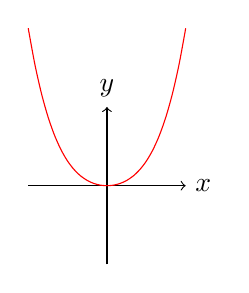
\begin{tikzpicture} 
		\draw[->] ( - 1, 0 ) -- (1, 0 ) node[right] {$x$}; 
		\draw[->] (0, -1) -- ( 0, 1) node[above] {$y$}; 
		\draw[scale=1, domain=-1:1, smooth, variable=\x, red] 
			plot ({ \x}, {\x * \x * \x * \x + \x * \x  } );  
	\end{tikzpicture} 
	\quad 
	\begin{tikzpicture} 
		\draw[->] ( - 1, 0 ) -- ( 1, 0 ) node[right] {$x$}; 
		\draw[->] (0, -1) -- ( 0, 1) node[above] {$y$}; 
		\draw[scale=1, domain=-1:1, smooth, variable=\x, red] 
			plot ({ \x}, {\x * \x * \x * \x  - \x * \x  } );  
	\end{tikzpicture}

	\caption{ Here we've shown plots where $T > T_c$ on the left versus when $T< T_c$} 
\end{figure} 
In the case where $T > T_c $, our minimum point is at $m = 0$ as shown in the graph, which means that we have no average magnetisation. For this reason, we call this a disordered state. 
When $T < T_c$, we have that the system that settles at either minimum point. We can calculate this minimum point explicitly by differentiating by solving for $f'(m ) $ to get that our minimum points are 
\[ 
m_0 = \pm \sqrt{ \frac{ 3 ( T_c - T ) }{ T } } 
\] 
This is our first example of a phase transition; when a physical quantity (in this case, average magnetisation), depends discontinuously on some parameter. We define an nth order phase transition when the nth derivative of the equilibrium value is discontinous when we differentiate it by some parameter.In other words, when the function $f'(\mu) = f( \mu, m_0 )$ is discontinuous when we differentiate it n times with respect to $\mu$, then do we have a phase transition. In this example, if we substitute our values of $m_0$ back into $f$, then 
\[ 
f(m_0, T) = \begin{cases} 
		0 & T > T_c \\ 
		 - \frac{3}{ 4} \frac{ ( T - T_c)^2 }{ T }  & T< T_c 			\end{cases} 
\] 
At $ T = T_c$, we have that $f( m_0, T )$ and $\frac{ df }{ dT } $ are continuous, but we have a discontinuity at $\frac{ d^2 f}{ dT^2 } $. 
Thus, our phase transition is a second order phase transition. 
We can also see this discontinuity exhibited when we examine heat capacity. 

Our heat capacity is defined as our change in average energy as temperature changes
\[ 
\frac{ d \langle E \rangle }{ dT}  = c
\] 
But we can calulate average energy in terms of our partition function $Z$, which is given by 
\[ 
\langle E \rangle = \frac{ - \partial \log Z }{ \partial B} 
\] 
We use the chain rule to express derivatives in $T$ as derivatives in $\beta$
\[ 
\frac{d}{ dT} = \frac{ d \beta} { dT } \frac{ \partial }{ \partial \beta} =  - \beta^ 2 \frac{ \partial }{ \partial \beta} 
\] 
Hence our heat capacity is given by the formula 
\[ 
c = \beta^2 \frac{ \partial^2 \langle \log Z \rangle}{ \partial \beta^2 } \] 
Now, with our saddle point approximation, we know that 
\[ 
\log Z = - \beta N f(m_{min} ) \implies \log Z =  - \beta N f(m_{min}) = \begin{cases} 
0 & T > T_c \\
\beta N \frac{ 3}{ 4} \frac{ ( T - T_c)^2 }{ T^2 }  & T < T_c 
\end{cases} 
\]  
In the case when $ T < T_c $, we have that setting $T = 1 / \beta $ gives us that 
\[ 
\log Z = \frac{ 3}{ 4} N ( 1 - 2 T_c \beta + T_c^2 \beta^2 ) \implies c = \frac{3}{ 2} N T_c^2 \beta^2 
\] 
Hence, as $T \rightarrow T_c$, we have a discontinuity in our heat capacity \[ 
C = \begin{cases} 
0 & T \rightarrow T_c^- \\
\frac{3}{2} N & T \rightarrow T_c^+ 
\end{cases} 
\] 
Since this involves a discontinuity in a second derivative of $f(m_{min})$ ( in this case $\beta$ ), this is a second order phase transition. 


\subsubsection*{The case when $B \neq 0 $} 
Now, in the case where $B \neq 0$ and we have our free energy given by 
\[ 
f(m) =  - Bm + \frac{1}{ 2}( T - T_c )m^2 + \frac{T}{ 12} m^4 + \dots \] 
In the case where $T < T_c$, we already have two minimum points, but as the graphs show we have a global minimum at a specific point depending on the sign of $B$. This is shown in the graphs below, where when $B>0$ our equilibrium magnetisation lies at $m_0 > 0$, and when $ B < 0 $ our equilibrium magnetisation lies at at $m_0 < 0$. 

\begin{figure}[h]
\centering
\begin{tikzpicture}[scale=0.7]
\begin{axis}[ 
xlabel=$m$,
ylabel={$f(m)$}, 
axis x line=center,
axis y line=center,
ticks=none, 
no markers, 
clip=false 
] 
\addplot { -  5 * x - 2 *  x^2 + 0.5 *  x^4}; 
\end{axis}
\end{tikzpicture} 
\quad
\begin{tikzpicture}[scale=0.7]
\begin{axis}[ 
xlabel=$m$,
ylabel={$f(m)$}, 
axis x line=center,
axis y line=center,
ticks=none, 
no markers, 
clip=false  
] 
\addplot { +  5 * x - 2 *  x^2 + 0.5 *  x^4}; 
\end{axis}
\end{tikzpicture}

\caption{Our global minimum depends on the sign of $B$ this time} 

\end{figure} 

\subsection{A Brief look at Universality} 
Right now we'll explore a very strange phenomena in physics - the concept of universality which we mentioned in the introduction. Let's take a look at a different example of a phase transition - liquid and gas phase transitions given governed by the Van der Waals equation. We have the phase transition diagram as follows. 

From the Van der Waals equation, we also can look at limiting behaviour as $T \rightarrow T_c $, and we can derive critical exponents
\begin{align*} 
v_{gas}  - v_{liquid} & \sim (T - T_c)^\beta \\
v_{gas}  - v_{liquid } &  \sim (P - P_c)^{\frac{ 1}{ \delta } } \\
\end{align*} We can define compressiblity, 
\[ 
\kappa =  - \frac{1}{ \nu } \left.  \frac{ \partial \nu }{ \partial p } \right\vert_p 
\] 
We can show that \[ 
\kappa \sim \frac{1}{ (T - T_c)^{ \gamma} } , \quad \gamma  = 1 
\]
One can notice that these are the same exponents one can find from the Ising model, which is an interesting phenomenon! We say that in this case, the theory magnetisation and liquid-gas phase transitions are in the same universality class. To gain a rough intuition of why this might be true, we can also model gases as a lattice, where the energy cost of a particle being in a position costs an energy potential $\mu$, and the energy cost from a Van der Waals force of neighbouring particles is given by a coupling constant $J$. In this case, our energy is given by 
\[ 
E =  - 4J \sum_{ \langle ij \rangle} n_i n_i  - \mu \sum_i n_i
\] 
The variable 
\[ 
n_i = \begin{cases} 
	0 & \text{ if the lattice space isn't occupied } \\
	1 & \text{ if the lattice space is occupied } 
	\end{cases} 
\] can be mapped to spins with the map $ s_i = 2n_i - 1$, so that when $n_i = 1, s_i =1 $ and when  $n_i   = 0, s_i = -1$. 

\pagebreak 
\subsection{The Landau-Ginzburg approach} 
Now that we've covered using $m$ with the Ising model as an order parameter in Landau theory, we can generalise this a bit further. How do we modify this argument to move away from lattices and into a continuous space with some dimension say $\mathbb{R}^d$? If we could achieve this, then we would be able to make sense of expressions such as $m(\mathbf{x}), \quad \mathbf{x} \in \mathbb{R}^n$. 
\[ 
m \rightarrow m(\mathbf{x} ) 
\] 

To get started, we use something called a coarse-graining approach. Imagine we divide up the space $\mathbb{R}^d$ into a tiny gridframe work, and then assign some value $m_{\mathbf{i}}$ to each point in this tiny grid. We can then define 
\[
m(\mathbf{x}) = \frac{1}{N} \sum_{\mathbf{i}} m_\mathbf{i}
\] where we specifically average over the nearest neighbours, close to $\mathbf{x}$. Thus, our magnetisation is from $m \in ( -1, 1 )$. To this, we can come up with a heuristic for a partition function. We can sum up our field configurations to give our partition functions
\[ 
Z = \sum_{m ( \mathbf{x} )} \sum_{ \{ s_i \} | m ( \mathbf{x} ) } e^{  - \beta [ s_i ] }  = \sum_{ m ( \mathbf{x} )}  e^{ - \beta F ( m ( \mathbf{x} )) } 
\] The difference with this and what we did before is that we've added a local dependence on $m$, called this a function, and then summed over all field configurations which give this particular configuration. For this approximation to be valid, we require that these tiny grids which divide up our space are large enough to cover a large amount of atoms, but small enough so that we still have a notion of continuity when we move from grid to grid. 

We're ready to promote this concept tot he path integral formulation of the partition function, by replacing the sum with an integral. 
\[
\mathcal{Z} = \int \mathcal{D}m(\mathbf{x})e^{ - \beta F(m)}
\]
In line with our usual expressions for probabilities with partition functions, we can then calculate the probability of obtaining a certain field configuration as 
\[ 
\mathcal{P} ( m ( \mathbf{x} ) )  = \frac{ e^{  - \beta F( m ) } }{ \mathcal{Z} } 
\] 
The measure
\[
\int \mathcal{D}m 
\] is meant to denote an integral over all possible field configurations $m(\mathbf{x})$, is called doing a functional integral. Intuitively, this notation is justified because the sum we're doing can be rewritten as follows, where in the second sum we're summing over all points instead, and then configurations
\[ 
\sum_{ m ( \mathbf{x} )}   \simeq \sum_{ \mathbf{x}_i }  \sum_m m_i ( \mathbf{x}_i )  = \int dm_1( \mathbf{x}_1 ) dm_2 ( \mathbf{x}_2 ) \dots dm_m ( \mathbf{x}_m ) 
\] 
We can extend this even more to include $m$ being an n-dimensional vector instead of the scalar we've presented it to be here. In this case, it would our partition function would be of the form 
\[
\mathcal{Z} = \int \mathcal{D}  \mathbf{m}(\mathbf{x}) e^{ - \beta F(\mathbf{m})} 
\]

Okay great. Now, we're ready to try an 'construct' a theory based on some restrictions we have gained from our intuition about physical systems. by constructing a theory, we mean that we would like to construct a sensible $F ( m ( \ve{x } ) ) $, which is an integral of something.  We'll list out some guiding principles in this section. 

\subsubsection*{Locality} 
In our theory, we would only like to consider short range interactions between points in space. This means that essentially, magnetisations at different points in space shouldn't correlate with each other. This is the principle of \textbf{locality}. It means that essentially, our free energy can integrate over one variable at each specific point. This means that an expression of the form 
\[ 
F ( m ( \ve{x})) = \spint   f( m ( \ve{ x} )) 
\] are  allowed, but a function that integrates over different points simultaneously like 
\[ 
F( m ( \ve{x}) ) = \int d^d x d^d y  \, \, f ( m ( \ve{ x} ), m ( \ve{ y} ) ) 
\] is not allowed. Now, we did say that we can allow \textit{short range} interactions. How are these incorporated in the theory? Well, we can include gradients of $m  $, such as terms like $ \nabla m$, to encode nearest neighbour interactions. This is because philosophically, taking a gradient is like looking at the difference in magnetisation at close points on a lattice which has small spacing; 
\[ 
\pdif{ m }{ \ve{ x} }  = \lim_{ a \rightarrow 0 } \frac{ m ( \ve{ x} + a \hat{ \ve { x} })  - m ( \ve{ x} )  }{ a } 
\] 

\subsubsection*{Translational and Rotational Invariance} 
Physical systems should be agnostic of whether we move them around in a translation sense, or if we rotate them about. Physical quantities should remain the same; systems shouldn't have a preferred vector or orientation. With this in mind, a condition we impose is that our form of $F(\mathbf{m})$ should be \textbf{invariant} under transformations of the type 
\[
\mathbf{m} \rightarrow \mathbf{m}' = R \mathbf{m} 
\] where $R$ is some rotation or reflection in the group $O(n)$. This is because the nature of our critical phenomena should be invariant of the orientation it's in. We can't allow terms like $ \ve{ n} \cdot \nabla \ve{ m } $, for a fixed $\ve{ n} $, for example. 

Since we have that $R^T R = 1, \forall R \in O(n)$, it's likely that we're permitted terms of the form 
\[
\mathbf{m} \cdot \mathbf{m}, \quad \nabla \mathbf{m} \cdot \nabla \mathbf{m}, \quad m^4 \dots 
\]

\subsubsection*{$\mathbb{ Z}_2 $ invariance}
In the Ising model, we have that intuitively, our physics doesn't change if we swapped $\uparrow \rightarrow \downarrow$ and $\downarrow \rightarrow \uparrow$. This means that $\mathbb{ Z}_2 $ symmetry is manifest in our physical systems, which implies that terms in $F$ should be invariant under the transformation 
\[ 
m ( \ve{ x} ) \rightarrow  - m( \ve{   x} ) 
\]
\subsubsection*{Analyticity} 
In physics, we rarely have to deal with functions which are not well behaved everywhere. A function is \textbf{analytic} if it has a well behave Taylor expansion in our region of interest. This means that nice polynomial functions of our order parameter such as 
\[ 
m ( \ve{ x} )^2, \, ( \nabla m ( \ve{ x} ) )^2, \dots 
\] are okay. However, a term like 
\[ 
 \log ( m ( \ve{ x} ) ) 
\] is not since the Taylor expansion is not well defined at $m = 0$. 

\subsubsection*{The final form of a plausible free energy} 

This motivates us to write an expression for our free energy as 
\[	
F(m) = \int d^d x\,  \alpha_2 m^2 + \gamma (\nabla m)^2 + \alpha_4 m^4
\] where we're working to just quadratic order. 
We have a $\mu^2$ coefficient beside $m^2 $ since, comparing with our mean field approximation we worked through earlier, we need this to me positive for the quadratic cutoff to remain valid. I'll go into more detail about this later. If our coefficient was negative then we'd have an unstable point for our magnetisation. 

So far, we have a free energy which is a function of a function. Can we think of an 'extremal' function which minimises this quantity? Well, we can employ a similar approach we used in deriving the Euler-Lagrange equations, by perturbing the configuration $ m ( \ve{ x} ) \rightarrow m ( \ve{ x} ).  + \delta m  $. Doing this with our expression for free energy above, we get that 
\begin{align*} 
\delta F & = \spint 2 \alpha_2 m ( \delta m ) +  2\gamma \nabla m \cdot ( \delta \nabla m ) + 4 \alpha_4 m^3 ( \delta m ) \\
	&= \spint \delta m \left( \alpha_2 m + \alpha_4 m^2  - \gamma \nabla^ 2  m \right) 
\end{align*} 
Thus our functional derivative of the integrand is of the form 
\[ 	
\frac{ \delta f }{ \delta m } = \alpha_2 m + \alpha_4 m^3  - \gamma \nabla^2 m 
\] Thus, we have that if we want to find the field configuration $m ( \ve{ x} )$ which minimises the free energy, we need to solve the equation 
\[ 
\gamma \nabla^2 m = \alpha_2 m + \alpha_4 m^3 
\] One can easily check if we assume that $m $ is constant, we 3 possible solutions depending on the sign of $\alpha_2$. 
\[ 
\begin{cases} 
m = 0 & \alpha_2 > 0 \\
m = \pm \sqrt{ \frac{  - \alpha_2 }{ \alpha_4 } } & \alpha_2< 0  
\end{cases}
\] 

\subsection{Domain Walls}
However, we recognise that this obeys the same pattern as the mean field approximation! This is reassuring. However, we can go into a bit more detail, and explore field configurations in one dimension which smoothly move between $ \sqrt{ \frac{  - \alpha_2 }{ \alpha_4 } }$ and $  - \sqrt{ \frac{  - \alpha_2 }{ \alpha_4 } } $ (we can't have say, a step function because that means our gradient would be infinite). One can verify that a solution with this asymptotic property of converging to these stable state is given by 
\[ 
m = m_0 \tanh \left( \frac{ x - x_0}{ w }  \right), \quad W = \sqrt{ \frac{ 2 \gamma }{ \alpha_2 } } 
\] This is called a domain wall. 
We need to verify that this is a solution of the equation of motion.
We find that 
\[	\frac{d m }{dx } = \frac{m^{0 }}{W} \sech^2 \left( \frac{x - X}{W} \right), \quad \frac{d^2 m }{dx^ 2 } =  - \frac{2m_0 }{W^ 2 } \tanh \left( \frac{x - X}{W} \right) 	+ \frac{2 m_0 }{W^ 2} tanh^2 \left( \frac{x - X }{W} \right)   	\] 
However, we can just wrangle this into the form 
\[
\gamma \frac{d^ 2 m }{dx^ 2 } = - \frac{2 \gamma }{W^ 2 }m  +  \frac{ 2 \gamma }{W^ 2 m_{0 }^2 }m ^ 3 
\] If we substitute in our asymptotic values $ \pm m_{0 }$, as well as our characteristic width $W$, then 
we recover that indeed 
\[
\gamma \frac{d^ m }{dx^ 2 } = \alpha_2 m + \alpha_4 m^{3}
\] 
Now, we saw that the function $m $ has \textbf{ characteristic length} $ W$. Beyond this length 
we basically consider the function $ m $ to be constant. Let's try 
plug this function back into our expression for our free energy $ F ( m ( \vec{x}) ) $. 
Let's consider how the derivative terms scale first. Since the function is constant outside of our characteristic length, 
we need only to integrate in this range. Our free energy derivative term is 
\[
F_{deriv } ( m ) = \int d^{d} x \frac{1}{2 } \gamma ( \nabla m )^ 2 \sim L^{d -1 } \int dx \gamma \left( \frac{ d m  }{dx} \right)^2  
\] Let's take a look at what we've done here. We're approximating the 3d integral 
into an 'radial' component, 
and we've factored out a characteristic length scale of $L^{d - 1}$, much like 
when we do a spherical intgral in $ d$ dimensions, we take out a factor of 
$ S_{d -1 } $, the $ d - 1$ dimensional hypersphere, and leave in the 
radial integral. 
If we take just the constant term of $\frac{d m  }{ dx }$, then this integral 
becomes 
\[
 L^{d - 1} \gamma \int dx \frac{m_0^2 }{W^ 2}  \sim  L^{d - 1} \gamma \frac{m_{0}^2 }{W} \simeq L^{d -1 }\sqrt{\frac{ - \gamma \alpha_2^3 }{\alpha_4^3 }}  
\] We can also check that 
this is the characteristic length scale of other terms in the free energy. 

We can similarly do the polynomial functions in the free energy. 
We have, for the term with the $\alpha_2 $ coefficent, that 
\[
	F ( m ( \vec{v}) )  = \int d^{d }x \frac{1}{2 } \alpha_2( T ) m^ 2 \sim L^{d - 1} \int dx \frac{1}{2} \alpha_2 m^ 2
\] But again, we repeat the previous argument, 
and integrate just over the characteristic length scale $W$. 
Once again, we just take the constant terms, so that this 
is approximated by 
\begin{align*}
	L^{d - 1} W \alpha_2 m_{0}^2 &= L^{d - 1}\alpha_2W \sqrt{\frac{-\alpha_2}{\alpha_4}}  \\
	&= L^{d -1} W \frac{ - \alpha_2^2 }{\alpha_4 } \sqrt{\frac{ - 2 \gamma }{\alpha_4}}  \\
	& \sim \sqrt{ \frac{ - \gamma \alpha_2^3 }{\alpha_4 }} 
\end{align*}
Similarly, we have that our quartic term scales in this way. 
Hence, this free energy of a domain wall is well defined. 
The free energy of a domain wall $F_{DW}$, compared with the free energy of a ground state scales with a power law for characteristic length, 
\[ 
F_{ DW} \sim L^{ d - 1} \sqrt{ \frac{  - \gamma \alpha_2^3 }{ \alpha_4} } 
\] 
There's a special value of $d = 1$ since our domain wall has no length scale. 
This is what we call a critical dimension. 
Now, we can look at the probability of a domain wall occuring. 
As usual, the probability to have a certain field configuration is 
given by 
\[
	e^{  - \beta F ( m ) }
\] Hence, the probabilty of us having a domain wall at a given point $ x $ is 
\[
	\mathcal{  P}(\text{ domain wall at } x = X )  = \frac{e^{- \beta F_{wall}}}{\mathcal{ Z}}
\] Now, the first thing to notice is that when $ d= 1$, our exponential factor 
is constant since we have no length dependence. 
Overall, this constant is really small. Now, let's imagine 
we're in a section of  $ \R$ between $ \frac{L}{ 2} < x < \frac{L}{2}$. 
Then, we can calculate the probabability of us having a domain wall in this box. 
This means we'd like to calculate 
\[
	\int_{L / 2 }^{ L / 2 } dx \, \mathcal{ P }( \text{ domain wall at } X = x ) 
\] Naively, this looks like it'll just be $ L $ times the probability of a domain wall at a given point. 
However, we need to remember that domain walls have a characteristic length scale  $W$. 
This means we need to multiply by a factor of $ \frac{1}{ W} $ in the measure. 
So, we have that 
\[	\mathcal{ P }( \text{there's a domain wall between } \frac{L}{2 }< x < \frac{L}{2} )  = \frac{L}{W} \frac{e^{ - \beta F_{ wall}}}{ \mathcal{ Z }} 
\] What's the effect of having a domain wall in the range? 
Well, suppose that, in this one dimensional line, that we have a 
fixed magnetisation at the boundary, so suppose that $ m (  - \frac{L}{2 }) =  - m_{0 } $.
Then, the effect of a domain wall would be to flip this to $ m ( \frac{L}{2 })  = m_{ 0 } $ 
at the other end of the line. 

Now we can ask, if we have the condition that say $ m ( L / 2 ) = m_0 $, 
then what's the total probability of the magnetisation staying the same, 
or switching, by the time we get to the other side? 
The simplest way to find out what's happening is to consider 
the probability that we have $ N $ domain walls appearing in the system. 
Let's write down the expression first, then explain why this is. 
Our expression 
\[
	\mathcal{ P }\left( \text{ n domain walls}  \right)  = \frac{e^{ - n \beta F_{wall}}}{\mathcal{Z} W^n } \int_{L / 2}^{ L / 2 } dx_1 \int_{x_1}^{ L / 2 } dx_2 \dots \int_{ x_{n-1}}^{ L / 2} dx_n  
\] To see why this is, observe that, without loss of generality, we can place a domain wall anywhere
in the range, as the first domain wall to be placed. This is represented in the first integral. 
After that, we can place a wall any point after that wall, assuming 
its placed at the point $ x_{1}$. We repeat, to place a wall after that, and so on, 
until we've placed $n $ walls. 
Our probability density given by the exponential $ e^{ - \beta F_{wall}}$ is constant, so we
pull $ n $ of these factors out. 

An elegant argument to evaluate this integral is to observe that 
this term is symmetric amongst permutation of the variables $ x_1, x_2, \dots x_n $. 
So, we're essentially multiplying the first integral $ n $ times, 
but to take into account the permutation symmetry, we need to 
divide by $ n ! $. 
Thus 
\[
	\mathcal{ P }\left( \text{n domain walls} \right) = \frac{1}{n! \mathcal{ Z}} \left( \frac{L e^{ - \beta F_{wall}}}{ W} \right)^{n }   
\] Now that we've done this, calculating the probability of whether 
magnetisation will flip by the time it reaches the other side 
is simply a matter of looking at whether we have an odd or even 
number of domain walls. If we have an even number, 
our magnetisation flips an even number of times and thus is not changed. Hence, 
\[
	\mathcal{ P }( m_0 \to  m_0 )  = \sum_{n \text{ even }} \mathcal{P }\left( \text{n walls} \right) \frac{1}{\mathcal{Z}} \cosh \left( \frac{L e^{ - \beta F_{wall}}}{ W } \right)  
\] Similarly, our probability of switching sign is 
\[
	\mathcal{ P }( m_{0} \to   - m_0 ) = \frac{1}{\mathcal{ Z}} \sinh \left( \frac{L e^{ - \beta F_{wall}}}{ W} \right) 
\] What's the point of all this? 
Well, since our dimension was at $d = 1$, our probability diverges and $ L \to \infty $.
Thus, the probabilities $ \mathcal{ P }( m_0 \to  m _0 ) $ and $ \mathcal{P }( m_0 \to - m_0 ) $ 
are indistiuishable. 
We have a disordered state in one dimension, and hence mean field theory 
here breaks down. However, when 
$ d = 2$, we have that $ F \sim L $, so as we take the limit
as  $ L \to  \infty $, the terms don't diverge and we still retain an memory of 
the boundary conditions initially at $ x =  - \frac{L}{2}$. 


\pagebreak


\section{Evaluating Path Integrals and Gaussian Path Integrals }
We want to compute the path integral 
\[
	\mathcal{ Z} = \int \mathcal{D}m ( \vec{x}) e^ { - \beta F( m ( \vec{x}) ) } 
\] This object forms flutuations around the saddle point. 
This object is dominated around the saddle point (a weaklu coupled theory). 
Hence, we can work perturbatively. 
However, if the object was strongly coupled, the fluctuations matter just as much. 
If we set our magentic field to zero, we know our free energy takes the form 
\[
	F( \phi ( \vec{x}) )  = \int d^{d}x \left[ \frac{1}{2} \alpha_2(T ) \phi^2 + \frac{1}{4}\alpha_4(T) \phi^{4} + \frac{1}{ 2} \gamma( T ) ( \nabla \phi)^2 + \dots  \right] 
\] We can do a gross simplification here where we take $\alpha_4 \to 0 $.
To justify the following approximations, we need to keep track of what our 
\textbf{mean field} terms are. 
In the case where 
\begin{itemize}
	\item $\alpha_2 > 0 $, to leading order, our mean field is 
		\[
			\langle \phi \rangle  = 0
		\]  Since we're assuming that $\phi $ is close to zero, then 
		the quartic terms disappear. Hence, we're just left with 
		the quadratic and derivative terms. 
		\[
			F ( \phi( \vec{v}) ) = \int d^{d} x \frac{1}{2} \alpha_2 \phi^2 + \frac{1}{2 } \gamma ( \nabla \phi ) ^ 2  
		\] 
	\item In the case where $\alpha_2 ( T ) < 0 $, we redefine 
		$ hat{\phi }( \vec{v}) = \phi ( \vec{v})  - \langle \phi \rangle  $	


\end{itemize} 
There's a very good reason why we need to make a redefinition 
for the case where $\alpha_2 < 0 $. This is because, when we solve for the equations of motion, 
just as in the mean field case, we recover two constant solutions 
\[
 \left< \phi \right> = \pm m_0 = \pm \sqrt{ \frac{ - \alpha_2 }{\alpha_4 }} 
\] We get that $ \left< \phi \right> $ is not close to zero, but these
two equilibrium terms instead. 
In addition, it's obvious that if we just set the quartic terms to zero 
with $ \alpha_2 < 0 $, then the whole qualitative shape of our potential 
would be different: we would have an upside down smiley face.  
However, we can make a different field which is close to zero. We define a translated field
\[
	\widetilde{ \phi }( \vec{x})  = \phi ( \vec{x})  - \left< \phi \right>
\] These are small fluctuations around the mean field average. 
If we substitute these expressions into the free energy, we have
\[
	F( \widetilde{\phi}) = \int d^{d }x \frac{1}{ 2} \alpha_2 ( T ) ( \widetilde { \phi} + \left<\phi \right> )^ 2 + \frac{1}{4} ( \widetilde{ \phi} + \phi)^ 4 + \frac{1}{2 } \gamma ( \nabla  \widetilde{\phi} ) ^2 
\] Now, up to quadratic order, the constant terms from $ \left< \phi \right> $ 
come out to form the integral $ F ( \left< \phi \right> ) $. The non constant terms 
give a linear and quadratic integral as follows 
\[
	F = F( \left< \phi \right>) + \int d^{d } x \alpha_2 ( T ) \left< \phi \right>\widetilde{ \phi} + \alpha_4 \widetilde{ \phi } \left< \phi \right>^3 +\int d^{d } x \frac{1}{2} \alpha_2 ( T ) \widetilde { \phi }^2 + \frac{3}{2 } \left< \phi \right>^2 \alpha_4 + \frac{\gamma}{2 } ( \nabla \widetilde{ \phi }  )^2 
\] 
In the integral with terms linear in $ \widetilde{ \phi } $, the coefficient is 
 \[
\alpha_2 \left< \phi \right> + \alpha_4 \left< \phi  \right>^3 = 0, \quad \left< \phi \right> = \sqrt{ \frac{ - \alpha_2 }{\alpha_4}} 
\] Thus, the linear term vanishes, and we're left with a quadratic and derivative term
just like in the case with $ \alpha_2 < 0 $.
We can write the quadratic $ \phi $ coefficient as 
\[
	\int d^{d }x \frac{1}{ 2 } \alpha_2' ( T) \widetilde{ \phi }^2 
\]  where we have that 
\[
\alpha_2'  = \alpha_2 + \frac{3}{2} \left< \phi  \right>^2\alpha_4 = \alpha_2  - 3 \frac{\alpha_2 }{\alpha_4} \alpha_4  = - 2 \alpha_2 
\] 
Hence, in terms of our new translated field, we can write the free energy as 
\[
	F (\widetilde{ \phi } ) = F( \left< \phi \right>) + \int d ^{d }x \frac{1}{ 2} \alpha_2' \widetilde{ \phi } + \frac{1}{2 }\gamma ( \nabla \phi)^2 \dots 
\] 

We move into Fourier space with 
\begin{align*}
	\phi_{\vec{k}}  &= \int d^{d}x e^{ - i \vec{k} \cdot  \vec{x}} \phi( \vec{x}) \\
	\phi_{ \vec{k}}^*  &= \phi_{-\vec{k}}  \\
\end{align*}
However, recall that we've coarse grained, which means 
we have to put out some Fourier modes, by an ultraviolet cutoff. 
Inserting this expression into our free energy, we have that 
\[
	F [ \phi_{ \vec{k}} ] = \frac{1}{2}\int d^{d} \vec{k}_1 \int d^{ d}\vec{k}_2 
\] 
Given our form of free energy $F(m)$, our usual way of computing our partition function would be \[ Z = \sum_{\text{configurations}} e^{ - \beta F(m) } \] However, with coarse graining introduced, we now integrate over all possible configurations of $m = m(\mathbf{ x} )$. To do this, we introduce a measure called a path integral, and thus our partition functions is given by \[ Z = \int \mathcal{D} m \, e^{ - \beta F(m)} \]
Where the measure $\int \mathcal{ D } m $ is telling us to integrate over all possible field configurations. 

Question is, how do we even begin to evaluate this kind of object? The key is to rewrite this measure as a product of integrals of Fourier modes, that is, we diagonalise $m$ in Fourier space and rewrite \[ \int \mathcal{D}m  = \prod_\mathbf{k} \mathcal{K} \int d m_\mathbf{ k } d m^*_\mathbf{k} \] 
In what follows, we'll be using both continuous and discrete decomppositions of $m$ into Fourier modes. We decompose $m( \mathbf{x} ) $ into contnuous Fourier modes as \[ m(\mathbf{x} ) = \int  \frac{d\mathbf{k}}{ ( 2 \pi )^d }\, e^{ - i \mathbf{x} \cdot \mathbf{k}}m_\mathbf{k} \] and decompose $m$ into discrete Fourier modes in some volume $V$ as \[ m(\mathbf{x} ) = \frac{1}{ V} \sum_\mathbf{k} e^{ - i \mathbf{x} \cdot \mathbf{k} }m_\mathbf{k} \] 

At this point, as a result of our coarse graining proceduce, since we're counting averages over a lattice, we need to ensure that our Fourier modes aren't too high. So, we impose that 
\[
 \phi_{\vec{k}} =0, \quad  \frac{\pi}{ a } < \| k \|  
\] Where $ a $ is the characteristic length of our coarse graining procedure. 

If we rewrite our free energy $F (m)$ in terms of our Fourier modes, we have \[ F(m) = \int \frac{d m_\mathbf{k_1} d m_\mathbf{k_2}d^d x}{( 2\pi )^d} \, \left( \mu^2 m_{\mathbf{k}_1} m_{\mathbf{k}_2} e^{ - i \mathbf{k}_1 \cdot \mathbf{x} } e^{ - i \mathbf{k}_2 \cdot \mathbf{x} } - \mathbf{k}_1 \cdot \mathbf{k}_2 e^{ - i ( \mathbf{k}_1 + \mathbf{k}_2  \cdot \mathbf{x} )}m_{\mathbf{k}_1} m_{\mathbf{k}_2} \right) \] 

At this point, it's useful to remember the identity \[ ( 2 \pi )^d \delta (\mathbf{k} ) = \int d^d x e^{- i \mathbf{x} \cdot \mathbf{k}} \] so our final expression for our free energy is \[ F(m ) = \int \frac{ d \mathbf{k} }{ (2 \pi ) ^d } \left( \mu^ 2 |\mathbf{k} |^2 + \alpha \right) m_\mathbf{k} m_{ - \mathbf{k} } \]   
Substituting this transformed expression for our free energy, and using our measure which is the product of Fourier modes, our partition function \[ Z = \left( \prod_\mathbf{k} \mathcal{K} \int dm_\mathcal{k } dm_{ - \mathcal{k} } \right) \exp \left(  - \beta \int \frac{ d\mathbf{k} } { (2 \pi )^d } \left( \mu^2 |\mathbf{k}|^2 + \alpha \right) m_\mathbf{k} m_{ - \mathbf{k}} \right) \]
Now the tricky part is to somehow get rid of that integral over $d \mathbf{k}$ in the exponent. To do this, we discretize the integral over the possible modes $\mathbf{k} $ in a finite volume and then take this volume to infinity. \[ \int d \frac{ \mathbf{k} }{ (2 \pi)^d } f( \mathbf{k} ) = \lim_{V \rightarrow \infty} \frac{ 1 }{ V} \sum_\mathbf{k} f(\mathbf{k} ) \] where in this case in the finite volume, our modes $\mathbf{k} $ are appropriately quantized. This makes our integral above easier to hande because now we can write it as \[ \left( \prod_\mathbf{k} \mathcal { K } \int dm_\mathbf{k} dm_{  - \mathbf{k} } \right) \exp \left( - \frac{ \beta}{ V } \sum_{ \mathbf{ k } } ( \mu^2 |\mathbf{ k} |^2 + \alpha )m_\mathbf{k} m_{ - \mathbf{k} } \right) \] but we can factor out our above expression over the product so that \[ Z = \prod_{ \mathbf{k} } \mathcal {K} \int dm_\mathbf{k} dm_\mathbf{-k} \exp \left(  - \frac{1}{ TV}  ( \mu^2 |\mathbf{k}|^2 + \alpha ) m_\mathbf{k} m_\mathbf{ -k } \right) \] 
(There's a factor of 2 missing here which I need to correct). How do we go about evaluating this object? Well, recall that in a fourier transform, our negative fourier mode is indeed just the complex conjugate of the corresponding positive mode: 
\[ 
dm_{  - \mathbf{k}}  = dm_\mathbf{ k}^* 
\] 
So to do the above, we need to think carefully about how we integrate expressions that look like 
\[ 
\int dx dx^* \exp \left(  - \frac{ |x|^2 }{ 2 \alpha } \right)  
\] 
At first glance, one might think to treat the $x, x^* $ variables here separately and integrate twice over, but since $x$ clearly depends on $x^*$, we have that the expression above is just the same as integrating 
\[ 
\int dx \exp \left(  - \frac{ |x|^2 }{ 2 \alpha } \right) = \sqrt{ 2 \pi \alpha }  
\] 
This is our usual expression for a Gaussian-like integral. Our expression for our partition function is therefore 
\[ 
Z = \prod_{ \mathbf{k}} \sqrt{ \frac{ 2 \pi V T \mathcal{ K }^2 }{ ( \mu^2 |\mathbf{ k} |^2 + \alpha  ) } }  
\]   
where, in calculating this, we've pulled the constant $\mathcal{K}$ inside the square root to make our calculations with it easier later on. Now that we have our partition function, we're in good shape to start calculating quantities of interest. The most obvious one we can compute is our thermodynamic free energy, $F_{thermo} =  - T \log Z$. What we'll do now is naively plug our expression for $Z$ in, but then make an approximation to get it into a nice integral form. We'll work instead with the thermodynamic free energy per unit volume. 

This is given by
\[ 
\frac{ F_{ thermo} }{ V} =  - \frac{ T}{ V} \log Z =  - \frac{ T}{ 2V } \sum_{ \mathbf{k}} \log \left( \frac{ 2 \pi  V T \mathcal{K}^2 }{ ( \mu^2 |\mathbf{k}|^2 + \alpha ) } \right) 
\] 

But, we can do even better than this. Previously, we swapped out our integral for a sum, but now we can do the opposite thing and swap out our sum $\frac{ 1}{ V } \sum_\mathbf{k} $ with $\int \frac{ d^d \mathbf{ k} } { ( 2 \pi)^d } $. This gives the condensed expression that 
\[ 
\frac{ F_thermo}{ V} = - \frac{ T}{ 2} \int \frac{ d^d k}{ ( 2\pi )^d } \, \log \left( \frac{ 2 \pi V T \mathcal{K}^2 } { (\mu^2 |\mathbf{k}|^2 + \alpha ) } \right)  
\] 

In the $\mathbb{ C} $ case, we have 
\[
	\mathcal{ Z}_{\mathbb{ C} } = \prod_{\vec{k}}^{\infty} \left\{ \int d \phi_{\vec{k} }^r d\phi_{\vec{k} }^I e^{  - \frac{\beta}{2 V  } ( \gamma k^ 2 + \mu^ 2 )( \phi_{ \vec{k} }^ { r 2 }   + \phi_{\vec{k} }^{ I 2 }}  \right\}   
\] 
Our Gaussian integral identity implies that 
\[
	\mathcal{ Z}_{\mathbb{ C} } = \prod \mathcal{ N } \frac{ 2 \pi T V }{ \gamma k^ 2+ \mu^2 }  
\] So, in the real case we have that for the real field, 
 %\[
%	\mathcal{ Z } = \prod_{\vec{k}} N \left( \frac{ 2 \pi T V }{ \gamma k^2 + \mu^2 }  \right)^{ \frac{1}{2 } }    
%\] This is because our factors of $ d \phi_\vec{k}$ and $ d \phi_{  - \vec{k}}$ are now
related in the real case. 
Our free energy was $ \mathcal{ Z } = e^{  - \beta F_{ thermo  } }$. This means that 
in the discrete case 
we have that 
\begin{align*}
	\frac{F_{thermo  } }{V } &=   - \frac{T}{V} \log ( \mathcal{ Z })  \\
				 &=   - \frac{T}{ 2V } \sum_{ \vec{k} } \log \left( \frac{ 2 \pi T V N^2 }{ \gamma k^ 2 + \mu^  2} \right)  \\
				 & \sim  - \frac{T}{2 }\int d^{ d } k \frac{ 1 }{ ( 2\pi )^d } \log \left( \frac{ 2 \pi T V N^2  }{ \gamma k^2 + \mu^ 2 } \right) 
\end{align*}

For Heat capacity, we define 
\begin{align*}
	c &=  \frac{C}{V } \\
	  &=  \frac{\beta^2}{V  } \frac{\partial^ 2 }{\partial \beta^2 } \log ( \mathcal{ Z })  \\
	  &=  \frac{1}{2 } \left( T^2 \frac{\partial ^2 }{\partial T^ 2}  + 2T \frac{\partial  }{\partial T }  \right) \int \frac{d^{ d }k }{ ( 2 \pi ) ^ 2 } \log \left( \frac{ 2 \pi T V N^ 2 }{ \gamma k^ 2 + \mu^ 2 } \right)  \\
\end{align*} 
When we do this integral we get that 
\[
	c = \frac{1}{2 } \int_0^{ \lambda }  \frac{ d^{ d }k }{ ( 2 \pi ) ^  2} \left[ 1 - \frac{ 2T }{\gamma k^ 2 + \mu ^ 2 } + \frac{ T^ 2 }{ ( \gamma k^2 + \mu^ 2 )^ 2 } \right] 
\] The last two terms depend on dimension $ d $.
Here, we've added a cutoff from our lattice spacing approximation. 
Our middle term is 
\[
 \int_{ 0 }^\lambda dk \frac{ k^{ d - 1 } }{\gamma k^2 + \mu^2 } = \begin{cases}
 \lambda^{ d - 1} & d > 2 \\
 \log ( \lambda ) & d = 2 \\
 \frac{1}{\mu} & d =1 
 \end{cases} 
\] Our last term gives 
\[
	\int_{ 0 }^\lambda dk \frac{k^{ d - 1 }  }{ ( \gamma k ^ 2+ \mu^ 2)^ 2  } = \begin{cases}
		\lambda^{ d - 1} & d > 4 \\
		\log ( \lambda ) & d = 4 \\
		\mu^{ d - 4 } & d < 4 
	\end{cases}
\] For the case that $ d < 4 $
 \[
 c \sim | T - T_c |^{ - \alpha}, \quad \alpha  = 2 - \frac{d}{2 }
\] 

\subsection{Correlation functions} 
In mean field theory, we had no local specific information. 
\[
	\left< \phi ( \vec{x} )  \right> =  \begin{cases}
		0 & T > T_c \\
		\pm m_0 & T < T_c 
	\end{cases}
\] Our next simplest way to think about correlations is
\[
	\left< \phi ( \vec{x} ) \phi ( \vec{y} )  \right>
\] this tells us how fluctations propagate throughout time by encoding spatial
variations at multiple points. A naive way to 
think about this is how waves propagate in the material. 
Moreover, we can think about functions deviating from the mean
as the \textbf{connected correlation function}. 
This is defined as 
\[
	\left< \phi ( \vec{x} ) \phi( \vec{y} )  \right>_c = \left< \phi( \vec{x} ) \phi ( \vec{y} )  \right> - \left< \phi  \right>^2 
\] This is also known as the cumulant in statistics. 
We can compute these correlation functions explicitly. 

If we define 
\[
	F[ \phi ( \vec{x} ) ] = \int d^{  d} x \left[ \frac{\gamma}{2 } ( \nabla \phi)^ 2 + \frac{\mu^2 }{2 } \phi^2 + B ( x) \phi  \right] 
\] with the partition function 
\[
	Z [ B ( x) ] = \int \mathcal{ D } \phi e^{  - \beta  F [ \phi ( \vec{x} ), B ( \vec{x} ) ]}
\] We can take a functional derivative to get
\[
	\frac{1}{\beta } \frac{\delta \log \mathcal{ Z }}{\delta B ( \vec{x} ) } = \frac{1}{\beta \mathcal{ Z }} \frac{ \delta \mathcal{ Z }}{ \delta B ( \vec{x} ) }
\] However, this term, the benefit of doing this is that differentiating by $B ( \vec{v} ) $ pulls out a factor of $ \phi $ in the integral. Hence, the quantity we've calculated is 
\[
	- \frac{1}{\mathcal{ Z } } \int \mathcal{ D } \phi ( \vec{x})  e^{  - \beta F[ \phi , B  ] } =  - \left< \phi ( \vec{x} )  \right> \mid_{ B }
\] So, we've found a neat way to encode the average function in our partition function. 
This is exactly the same as encoding our average magnetisation 
in our partition function using mean field theory earlier. 
We can get even more information from this. We calculate an object called the \textbf{two-point} function. 
In analogy to moment generating functions in statistics, 
differentiating this a second time enables us to get the connected 
correlation function we listed earlier. If we act on what we have 
with $  \frac{ \partial  }{ \beta \partial  }$, the product rule gives us 
\[
	\frac{1}{ \beta ^ 2 } \frac{\delta^ 2   \log \mathcal{  Z} }{\delta B ( \vec{x} ) \delta B ( \vec{y} ) } = \frac{1}{ \beta ^ 2 \mathcal{ Z } } \frac{ \delta ^2 \mathcal{ Z } }{\delta B ( \vec{x} ) \delta B ( \vec{y} ) }  - \frac{1}{ \beta ^ 2 \mathcal{Z } ^ 2 } \frac{ \delta \mathcal{ Z } }{ \delta B ( \vec{x} ) } \frac{ \delta \mathcal{ Z } }{ \delta B ( \vec{y}) } 
\] This was obtained by applying the product rule on $ \frac{1}{ \mathcal{ Z } } $ as 
well as the derivative terms. 
The upshot is that the first term pulls down two factors, $ \phi ( \vec{x} )  $ and $ \phi ( \vec{y} ) $ from our free energy. 
Hence, our first term is 
\[
	 \frac{1}{ Z }\int \mathcal{ D } \phi \, \phi ( \vec{x} ) \phi ( \vec{y} ) e^{  - \beta F } = \left< \phi ( \vec{x} ) \phi ( \vec{y} )  \right>\mid_B
\]  Further more, observe that the second term is just 
$ \left< \phi  \right>^ 2 $. 
Thus, our final correlation function can be written in the compact form, writing our subscript $ B $ to denote evaluation at the field configuration $ B $, 
\[
	\left< \phi ( \vec{x} ) \phi ( \vec{y} )  \right>_c  = \frac{1}{\beta ^ 2 } \frac{ \delta ^ 2 \log \mathcal{ Z } }{\delta B ( \vec{x} ) \delta B ( \vec{y} ) } = \left< \phi ( \vec{x} ) \phi_( \vec{y} )  \right>_B - \left<\phi( \vec{x} ) \right>_B \left< \phi( \vec{y} )  \right>_B 
\] Now, above the critical temperature $ T > T_{  c} $, we have that our average 
magnetisation is given by $ \left< \phi ( \vec{x} )  \right>  = 0 $ when $B = 0$. 
Thus, we can condense what we have even further by 
 \[
	 \frac{1}{ \beta ^ 2 } \frac{ \delta ^ 2 \log \mathcal{ Z }  }{\delta B ( \vec{x} )  \delta B ( \vec{y} ) }\mid_{ B  =0 } \left< \phi ( \vec{x} )\phi ( \vec{y} )   \right>_{ B = 0} 
\] 


\subsection{Computing Gaussian Path Integrals}

\subsubsection{Our correlation function is just a Green's function} 
The point of this whole section is to drive the point home 
that diagonalising in Fourier space makes things easier!

Our total free energy, including the magnetic field, was
 \[
	 \int d^ d x \, \frac{\gamma}{2 } ( \nabla \phi ) ^ 2 + \frac{1}{2 }\mu^ 2 \phi ^ 2 + B ( \vec{x} ) \phi 
 \] Now, we already know that the Fourier expansion of the first two terms gives us an intergal in Fourier space which is equal to 
 \[
	 \int \frac{ d^ d k}{ ( 2 \pi ) ^ d } \left[  \frac{1}{2 } \left(  \gamma k^ 2 + \mu^ 2  \right) \phi_{ \vec{k} } \phi_{  - \vec{k} }   \right] 
 \] Now, to incorporate our magentic field, we just expand out $ \phi $ in Fourier modes 
 and sub in our definition for what a Fourier mode is for $ B $. 
 So, 
 \[
	 F_{ mag } = \int d^ d x \, \frac{ d^ d  k }{ ( 2 \pi ) ^ d } e^{  - i \vec{k} \cdot  \vec{x} } \phi_{ \vec{k}  } B ( x )
 \] Defining 
 \[
	 B_{ \vec{k}}  = \int d^d x \, e^{  i \vec{k} \cdot  \vec{x} } B ( \vec{x} ) \implies F_{ mag } = \int \frac{ d ^ d k }{ ( 2 \pi ) ^ d  } \, B_{ - \vec{k} } \phi_{ \vec{k}}
 \] Hence, our whole expression for our free energy in terms of 
 Fourier modes is 
 \[
	 F  = \int \frac{ d^ d k }{ ( 2 \pi ) ^ d } \left[  \frac{1}{2 }( \gamma k ^ 2 + \mu ^ 2 ) \phi_{\vec{k} } \phi_{  - \vec{k} } + B_{ - \vec{k} } \phi_{ \vec{k}} \right] 
 \] To evaluate this, we can define a translated integral as 
\[
 \tilde{\phi}_{\vec{k}} = \phi_{ \vec{k} } + \frac{B_{ \vec{k} }}{\gamma k ^  2+ \mu^ 2 } 
\] With this transformation, we can write 
\[
F [ \tilde{ \phi_{ \vec{k} } }] = \int \frac{ d^ d k }{ ( 2 \pi ) ^ d } \left[  \frac{1}{2 } ( \gamma k^ 2 + \mu ^ 2 ) | \tilde{\phi }_{ \vec{k}} |^ 2 - \frac{1}{2 } \frac{ | B_{ \vec{k} } | ^ 2  }{ \gamma k ^ 2 + \mu ^ 2 }  \right]   
\] Since we have that our partition function is given in terms of Fourier modes 
\[
 \mathcal{ Z } = \prod_{ \vec{k}} d \phi_{ \vec{k} } d\phi_{ - \vec{k} } e^{  - \beta F_{ thermo}}
\] Our Jacobian doesn't change because we're just changing by a constant. 
\[
	\mathcal{ Z } [ B_{ { k } } ] = e^{  - \beta F_{ thermo } }e^{ \frac{\beta}{2 } \int \frac{ d^ d k }{ ( 2 \pi ) d } \frac{ | B_{ \vec{k} } | ^ 2 }{\gamma k^ 2 + \mu ^ 2 }}
\] However, we can do an inverse Fourier transform 
\[
	\mathcal{ Z  } [ B ( \vec{x} ) ] = e^{  - \beta F_{ thermo }} e^{ \frac{\beta}{2} \int d^ d x d^ d y  B ( \vec{x} ) G ( \vec{x} - \vec{y} ) B ( \vec{y} )  } 
\]  We define our Green's function as 
\[
	G ( \vec{x} - \vec{y} ) = \int \frac{ d ^ d k }{ ( 2 \pi ) ^ d } \frac{e^{  - i \vec{k} \cdot ( \vec{x} - \vec{y} ) }}{\gamma k^ 2 + \mu ^ 2 } 
\] Differentiating twice, we get that
\[
	\left< \phi ( \vec{x} ) \phi ( \vec{y} )  \right>_{ B = 0 } = \frac{1}{\beta } G ( \vec{x} - \vec{y} )	
\]This is because
\[\frac{1}{\beta } \frac{\delta \log \mathcal{ Z}}{\delta B ( \vec{x} ) } =  \frac{1}{ B \mathcal{ Z } }e^{  - \beta F_{ thermo } } \frac{\beta}{2 } \left(  \frac{ \delta }{ \delta B ( \vec{x} ) } \int d^ d x d^ d y \, B ( \vec{y} ) G( \vec{x} - \vec{y} ) B ( \vec{x} )   \right) \text{exp} ( K ( B ( \vec{x} ) ) )  \]
Where we have defined for brevity that 
\[
	K ( B ( \vec{x} ) ) = \frac{\beta  }{2 }\int d^ d x d^ d y \, B ( \vec{x} ) G ( \vec{x} - \vec{y} ) B ( \vec{y} ) 
\] 
\subsubsection{An aside on functional integrals} 
Our functional derivative with respect to $ B ( \vec{x} ) $ kind of looks like if we were differentiating
$ B ^2 G $. 
Let's recall how to do a functional integral, from the persepctive of deriving the 
Euler-Lagrange equations from a quadratic free integral. Suppose we had 
an expression 
\[
	F ( B ( \vec{x} ) ) = \int d^ d z f ( B ( \vec{z} ) ) 
\] Then, our functional integral in the function $ g ( B ( \vec{x} ) ) $ 
that we get when we vary $ F $ with respect to $ B \to B + \delta B $, such that 
 \[
	 \delta F = \int d^ d z \delta B ( \vec{z} ) ( g ( B ( \vec{z} ) ) ) 
\] We did this before in deriving our equations of motion associated 
with our quadratic terms of our free energy. Varying with respect to 
$ \phi $, 
\begin{align*}
	\frac{ \delta F }{ \delta \phi } &=  \int d^ d x \, \gamma ( \nabla  \phi ) \delta ( \nabla  \phi ) +\mu ^ 2   \phi \delta \phi  \\
					 &=  \int d^ d x \, \gamma ( \nabla  \phi ) \nabla  ( \delta \phi ) + \mu ^ 2  \phi \delta \phi \\
					 &= \int d^ d x  - \gamma \delta \phi \nabla ^ 2 \phi + \mu ^ 2 \phi \delta \theta \\
					 &=  \int d^ d x \, \delta \phi ( - \gamma \nabla  ^ 2 \phi + \mu ^ 2 \phi ) 
\end{align*} Thus, in this case 
we have that our functional derivative is given by 
\[
 \frac{ \delta F  }{ \delta \phi } = - \gamma \nabla  ^ 2 \phi + \mu ^ 2 \phi 
\] 
As we shown in the previous section, solving this equation for 
$ \frac{ \delta F }{ \delta \phi }  = 0 $, gives us the most likely field configuration.
Thus, applying this to our previous problem an setting 
\[
	F = \int d^ d x \, \int d^ d y \, B ( \vec{x} ) G ( \vec{x} - \vec{y} ) B ( \vec{y} ) \implies \delta F = 2 \int d^ d x \,  \delta B ( \vec{x} ) \int d^ d y \, G ( \vec{x} - \vec{y} ) B ( \vec{y} )  
\] So, taking our functional derivative has left us 
with the term, relablleling variables, that  
\[
	\frac{ \delta F }{ \delta B ( \vec{x} ) } = 2 \int d^ d z \, G ( \vec{x} - \vec{z}) B ( \vec{z} )  
\] Hence, our expression for our first derivative of the log of the 
partition function simplifies to 
\[
	\frac{1}{ \beta } \frac{ \delta \log \mathcal{ Z } }{ \delta B ( \vec{x} ) } = \int d^ d z \, G ( \vec{z} - \vec{x} ) B ( \vec{z} ) 
\] If we differentiate this object using a functional derivative with respect to 
$ B $ again, we get that 
\[
	\frac{1}{ \beta ^ 2 } \frac{ \delta ^ 2 \log \mathcal{ Z } }{ \delta B ( \vec{x} ) \delta B ( \vec{y} ) } = \frac{1}{ \beta } G ( \vec{x} - \vec{y} ) = \left< \phi ( \vec{x} ) \phi ( \vec{y} )  \right> 
\] So, our correlation is a Green's function 
with a factor of $ \frac{1}{ \beta  }$. This 
is reminiscnent of quantum field theory, where our Feynman propagator 
was also essentially a Green's function. 
So, to calculate this correlation function, all we have to do 
is calculate this Green's function explicity. 


\subsubsection{Evaluating our Green's function} 
In the section that follows, we'll use symmetry arguments 
as well as a saddle point approximation to calculate the Green's function 
\[
	G ( \vec{x} ) = \int \frac{ d^ d k }{ ( 2 \pi ) ^ d } \frac{ e^{ i \vec{k} \cdot  \vec{x}  }}{ \gamma k^2 + \mu ^ 2 }
\] By rotational symmetry we can evaluate this Green's function as 
a function of $ r $, the magnitude of our vector 
\[
	G ( r)  =\frac{1}{\gamma } \int \frac{ d^ d k }{ ( 2 \pi ) ^ d } e^{  - i \vec{k} \cdot  x } \frac{1}{ k^ 2 + \frac{1}{ \zeta ^ 2 }}
\] We've defined our correlation length $ \zeta^ 2 = \frac{ \gamma }{ \mu^ 2 }$, which 
is a convenient scaling parameter, which we'll analyse the properties of later.  
We now use a fairly obvious identity to help us evaluate this intergal; we use 
the simple fact that 
\[
	\frac{1}{ k ^ 2 + \frac{1}{ \zeta ^ 2} } = \int_0^\infty dt e^{  - t ( k^ 2 + \frac{1}{\zeta ^ 2} ) }
\] The upshot of writing things this way allows us 
to nest the integrals within one another. Hence, we have that  
\begin{align*}
	G ( r) &=  \frac{1}{\gamma} \int \frac{d^ d k }{ ( 2 \pi ) ^ d } \int_0^\infty e^{  - t ( k^ 2 + \frac{1}{\zeta ^ 2 }) - i \vec{k} \cdot  \vec{x} } \\
	       &=  \frac{1}{\gamma } \int \frac{d^ d k }{ ( 2 \pi ) ^ d } \int_0^\infty dt \, dt e^{  - t ( k + \frac{ i x }{2t  })^ 2 }e^{  - \frac{r^ 2 }{ 4t }  - \frac{t}{\zeta^ 2 }} \\
	       &=  \frac{1}{\gamma } \frac{1}{4 \pi )^{ d / 2}} \int_0^\infty dt \, t ^{  - \frac{d}{2 } } e^{  - \frac{r^ 2 }{ 4t }  - \frac{t}{\zeta^ 2 }} \\
\end{align*}
Here we've used the fact that 
\[
	\frac{ d^ d k }{ ( 2\pi ) ^ d } \to \frac{ d \Omega_d }{ ( 2 \pi ) ^ d} k^{ d - 1 } dk, \int \frac{ d \Omega_d }{ ( 2 \pi ) ^ d }  = 2 \pi^{ \frac{d}{ 2}} \Gamma^{ -1} ( \frac{d}{2 } ) 
\] We can now employ the saddle point approximation 
\[
	G ( r) \simeq \int_0^\infty dt e^{ - S( t ) }, \quad S( t ) = \frac{r^ 2 }{ 4t } + \frac{t}{\zeta^ 2 }+ \frac{d}{ 2 }\log ( t) 
\]  Now, expanding the exponential about the minimum point, 
\[
	S( t) = S( t^* ) + \frac{ S'' ( t^ * ) t^ 2 }{ 2 } + \dots, \quad t^ * = \frac{\zeta^ 2 }{2 } ( - \frac{d}{2 } + \sqrt{ \frac{d^2}{4 } + \frac{r^2}{\zeta}} 
\] So, we have that 
\[
	G ( r) \simeq \sqrt{ \frac{ \pi }{ 2 S'' ( t^ * ) }}e^{  - S( t^ * ) } 
\] We now examine the limits in two regimes. 
\[
	r \gg \zeta, t^ * \simeq r \frac{\zeta}{2 } \implies G ( r) \sim \frac{1}{\zeta^{ \frac{d - 3 }{2 }}} \frac{ e^{  -\frac{r}{2 }}}{r^{ \frac{d - 1 }{ 2}}}
\] On the other hand, in the other regime 
\[
	r \ll \zeta, t^ * \simeq \frac{r^ 2 }{ 4 d } \implies G ( r) \sim \frac{1}{r^{ d - 2 }}
\] Recall, $ G( r) = \left< \phi( \vec{y} ) \phi ( \vec{x} )  \right> $
\pagebreak 

\section{Green's functions} 
Consider a multi-dimensional Gaussian integral: 
\[
I = 	\int_{ - \infty } ^ \infty d^ n y \, e^{ - \frac{1}{2 } y^ T  \cdot   G^{ - 1 } \cdot  y  }
\] Notice that we can diagonalise this object 
in the eigenbasis to give that 
\[
	I = det ^{ \frac{1}{ 2}  } ( 2\pi G ) 
\] Similarly, we can add a 'source' term to the integral and shift the variables to get
\[
	I_{ B } = \int_{ - \infty } ^ \infty d^ n y \, e ^{ - \frac{1}{2 } y \cdot  G^{ -1 } \cdot  y + \vec{B} \cdot  y } = det ^{ \frac{1}{2 } } ( 2 \pi G ) e^{ \frac{1}{2 } \vec{B} ^ T \cdot  G \cdot  \vec{B}}
\] From this result our expression for free energy 
\[
	F [ \phi ( \vec{x} ) ] = \int d^ d x\, \left[  \frac{1}{2 } \gamma ( \nabla \phi ) ^  2 + \frac{1}{2 } \mu ^ 2 \phi ^ 2 + \vec{B} \phi  \right]  
\] can be rewritten by parts with a dummy integral so that 
\[
	F [ \phi ( x) ] = \int d^ d x \, d^ d y \, \frac{1}{2 } \phi ( \vec{x} ) G ^{ -1 } ( \vec{x}, \vec{y} ) \phi ( \vec{y} ) + \int d^ d x\, \vec{B} ( \vec{x} ) \phi ( \vec{x} ) 
\] where we in this expression 
\[
	G ^{ -1 } ( \vec{x} , \vec{y} ) = \delta ^ d ( \vec{x} - \vec{y} ) ( - \gamma \nabla ^ 2_y + \mu ^ 2)  
\] We also have 
\[
	( - \gamma \nabla ^ 2 _ x + \mu ^ 2 ) G ( \vec{x}, \vec{y} ) = \delta^ d ( \vec{x} - \vec{y} ) , \quad G ( \vec{x}, \vec{y} ) = \int \frac{ d^ d k }{ ( 2 \pi ) ^ d } \frac{ e^{ - i \vec{k} \cdot ( \vec{x} - \vec{y} ) } }{\gamma k ^ 2 + \mu ^ 2 }
\] Be careful with inverting things! We need to integrate over them. 
Hence our correlation function satisfies a differential equation 
\[
	( - \gamma \nabla ^ 2 _ x + \mu ^ 2 ) \left< \phi ( \vec{x} ) \phi ( 0 )  \right> = \frac{1}{\beta } \delta^ d ( \vec{x} ) 
\] Away from the origin, this differential equation tells us that away from
the origin our fluctuations satisfy the Euler Lagrange equations. 
An aside on using Green's functions. 
If we have 
\[
	\mathcal{ O }( x) F( x) = H ( x) 
\] If we can solve $ \mathcal{ O } ( x) G ( x, y) = \delta ( x - y ) $, then setting
\[
	F ( x) = \int dy H ( y ) G ( x - y ) \implies \mathcal{ O }( x) F( x) = H ( x) 
\]
\subsection{Connection to Susceptibility} 
Let's apply these ideas to what we know about magnetic susceptiblity. 
Our equation that we've always used is 
\[
 \chi = \frac{\partial  m}{\partial   B } 
\] Now, we can promote this to a localised 
version by setting 
\[
	\chi ( \vec{x}, \vec{y} ) = \frac{\partial  \left< \phi ( \vec{x} )  \right> }{\partial B ( \vec{y} ) } = \beta ( \left< \phi ( \vec{x} ) \phi ( \vec{y} )  \right> \sim \int \mathcal{ D } \phi \frac{\partial \phi }{\partial  B } e^{  - \beta F [ \phi ] }  
\] From this local 
definition, we can define a global magnetic 
susceptibilty as 
\[
	\chi = \int d^ d x \chi ( \vec{x}, 0 ) = \beta \int d^ d x \left< \phi ( \vec{x} ) \phi ( \vec{y} )  \right>
\]
Recall our correlation function 
\[
	\left< \phi ( \vec{x} ) \phi ( \vec{y} )  \right> = \begin{cases}
		\frac{1}{r^{ d - 2}  } & r \ll \zeta \\
		e^{ - \frac{r}{2 } } / r ^{ \frac{ d -1 }{ 2 } } & r \gg \zeta
	\end{cases}
\] This implies that our critical exponents satisfy $ \mu ^ 2 \sim | T - T_{ c } | $, 
and $ \zeta \sim \frac{1}{ | T - T_{ c } | ^{ \frac{1}{ 2 }  } } $. 
Thus at low temperatures, our correlation length diverges, so 
our system because highly correlated. 

\subsection{Critical exponents} 
We say from our earlier argument that $ \zeta \sim \frac{1}{ | T - T _ c |^ \nu } , \nu = \frac{1}{2 } $ And, our correlation goes like
\[
	\left< \phi ( \vec{x} ) \phi ( \vec{y} )  \right> \sim \frac{1}{ r^{ d - 2 + \eta }} \quad \eta  =0 
\] So far, this agrees with our predictions for mean-field theory, 
but we still have some errors. 

\subsubsection{Upper critical dimension} 
In mean field theory, $ \left< \phi ( \vec{x} )  \right> = \pm m_0 $. 
But going into our path integral formulation, 
we ask how big are the fluctuations relative to $ m_0 $. 
If our fluctuations are very big, we shouldn't
expect our calculations to match our 
predictions from mean field theory. 
We look at our ratio
\[
	R = \frac{\int _ 0 ^\zeta d^ d x \, \left< \phi ( \vec{x} ) \phi ( \vec{y} )   \right>  }{\int_0 ^ \zeta d^ d x \, m_0 ^ 2 } \sim \frac{1}{m_0 ^ 2 \zeta ^ d } \int_0 ^ \zeta dr \, \frac{ r^{ d- 1} }{r^{ d - 2 } } \sim \frac{ \zeta^{ 2 -d } }{m_0 ^ 2 }
\]  
Now substituting in our critical exponents, 
\[
 m_0 \sim | T - T_c |^{ \frac{1}{ 2 } }, \zeta \sim | T -T _c|^{- \frac{1}{2 } } \implies R = | T -T_c | ^{ \frac{ d - 4 }{ 2 } }
\]

\subsubsection{Translating to Quantum Field Theory} 
We have many links between statistical field theory and
quantum field theory. 
\[
	\text{ SFT:  } \mathcal{  Z} = \int \mathcal{ D } \phi e^{ - \beta \int d^ d x \, F [ \phi ] }
\]  Here we have $ d $ spatial dimensions. 
In quantum field theory, 
we have that 
\[
	\mathcal{ Z } = \int \mathcal{ D } e^{ \frac{i}{\overline{h} } \int d^ d x \mathcal{ L ( \phi ) }}
\] Here we have $ d $ spactime dimensions, with an $ \frac{i}{\overline{h} }$ factor. 
We do a wick rotation $ \tau = i t $, 
so that our differential operator 
 \[
 \partial  _ t^ 2 +  \nabla ^ 2 \to \partial _ \tau ^ 2 - \nabla ^ 2 
\] Similarly, our path integrals transform as 
\[
	\mathcal{ Z  } = \int \mathcal{ D } \phi e^{ \frac{i}{\overline{h} } S [ \phi ]  } \to \mathcal{ Z } = \int \mathcal{ D } \phi e ^{ - \frac{1}{\overline{h}  } S_{ E } [ \phi ] }
\] So our quantum fluctuations are identified with thermal fluctuations.
$QFT_{ d -1 } \sim SFT_d $. 
\pagebreak 

\section{The Renormalisation Group}%
\label{sec:the_renormalisation_group}
The idea of the renormalisation group is an idea that 
was pioneered by Kadanoff, Fisher and Wilson which formalises
how physics changes depending on our scale. It's an important idea 
which helps explain universality

\subsection{Basic Introduction} 
Consider the free energy 
\[
	F [ \phi ] = \int d^ d x\,  \left[  \frac{1}{2 } ( \nabla \phi ) ^ 2 + \frac{1}{2 } \mu ^ 2 \phi ^ 2 + g \phi ^ 4 + \dots  \right] 
\] Recall that when we're writing this theory, 
we only used the few basic assumptions such as $ \mathbb{ Z} _ 2 $ symmetry, 
analyticity, and so on. 
So in essence, we could have included terms like 
$ g _{ 126} \phi ^{ 126 } $,  $ ( \nabla ^ 2 \phi ) ^ 2 $ and so on. 
These terms have coupling constants in front of them, 
such as $ \mu ^ 2 = T - T _ X $, which we call Wilson coefficients. 
We can also rescale our coupling coefficients so that we 
absorb $ \beta $ in our free energy, so we can write 
\[
	\mathcal{Z  } = \int \mathcal{ D } \phi \, e ^{  - F [ \phi ] }
\]  The final piece of the theory is that we also 
specificed some cutoff $ \Lambda $ such that 
\[
 \phi _{ \vec{k} } =0 , \quad  |  \vec{k} |  \geq \Lambda, \Lambda \sim \frac{\pi}{ a }
\] The crux of the renormalisation group 
is what happens when we ask what happens when we change $ \Lambda $? 
Since what we wrote down the most general theory to begin with, 
when we change  $ \Lambda  $ we expect the same form of theory 
but with different coupling constants. 
When we change the cutoff we call this a 'flow'. 

\subsection{Flowing to the 'IR' (long distances)} 
Imagine we only care about predictions at on scales
$ L \gg a $. Then, we can write a theory 
with a new cutoff given by 
\[
 \Lambda' = \frac{ \Lambda }{ \epsilon }, \quad \epsilon > 1 
\] This means that all fourier modes $ \frac{1}{ L } \leq | \vec{k} | \leq \Lambda $
We can expand Fourier modes as 
\[
\phi_{ \vec{k} }  = \phi_{\vec{k}}^-  + \phi_{ \vec{k} } ^ + 
\] The $ \phi_{ \vec{k} }^-$ are low frequency modes with 
\[
 \phi_{ \vec{k} }^ -  = \begin{cases}
	 \phi_{ \vec{k} } &  | \vec{k} | \leq \Lambda ' \\
	 0 & \text{ otherwise }
 \end{cases}
\] And our $ \phi_{ \vec{k} } ^ + $ are our high frequency 
terms with 
\[
 \phi_{ \vec{k} }^  +  = \begin{cases}
	 \phi_{ \vec{k}  } & \Lambda ' < \| \vec{k} \| < \Lambda \\
	 0 & \| k \| \geq \Lambda 
 \end{cases}
\]  
We can write out our free energy 
in terms of this fourier mode split, so that 
\[
	F [ \phi _{ \vec{k}  } ] = F_ 0 [ \phi_{ \vec{k} }^ - ]  + F_ 0 [ \phi_{ \vec{k} } ^ +   ] + F_ I [ \phi_{ \vec{k} } ^ + , \phi_{ \vec{k} } ^ - ]  
\]  The final term in this expression can be 
interpreted as an interaction between long and short length scales 
in the Fourier modes. 
We can then write out our partition function as
\[
	\mathcal{ Z} =  \int \prod_{ k <  \Lambda  } d \phi_{ \vec{k}} e^{  - F }  
\] However, the upshot of this is that 
now we can decompose $ F $ into the high and low frequency modes 
which we were derived earlier.
We have that
\[
	\mathcal{ Z } = \int \prod_{ k <  \Lambda ' } d \phi_{ \vec{k} }^- e^{  - F_0 [ \phi _{ \vec{k}} ^-]} \int \prod_{ \Lambda ' <  k < \Lambda} d \phi_{ \vec{k} } ^ + e^{  - F_ 0 [ \phi_{ \vec{k} } ^ +  ] } e^{  - F_ I [ \phi_{ \vec{k} } ^ + , \phi_{ \vec{k} } ^ - ]}
\] But the upshot of writing things out 
like this is that we can then write out an 'effective' 
action which only concerns integrals 
from our product of low frequency Fourier modes. In 
other words, we have that 
\[
	\mathcal{ Z } = \int d \phi_{ \vec{k}  } ^ - e^{  -F' [ \phi_{ \vec{k} } ^ -  ] }, \quad e^{  - F' [ \phi_{ \vec{k} } ^ - ]} = e^{ - F_ 0 [ \phi_{ \vec{k} } ^ -  ] } \int \prod_{ \Lambda ' < k < \Lambda } d \phi_{ \vec{k} } ^ +   e^{  - F_ 0 [ \phi_{ \vec{k} } ^ +  ] } e^{  - F_ I [ \phi_{ \vec{k} } ^ + , \phi_{ \vec{k} } ^ - ]}
\] 
%\begin{align*}
  % 	\mathcal{ Z } &=  \int \prod_{ \| k \| \le \Lambda ' }  e^{  - F_0 [ \phi_{ \vec{k} ^ -  }  ]  } \int \prod_{ \Lambda < k < \Lambda ' } d \phi_{ \vec{k} } ^ + e^{  - F_0 [ \phi_{ \vec{k} } ^ - ]   } e^{  - F_{ I } [ \phi_{ \vec{k} } ^ - , \phi_{ \vec{k} } ^ + ]}\\
% 	     &=  \int_{ k < \Lambda' } d \phi_{ \vec{k} } ^ - e^{  - F ' [ \phi_{\vec{k} } ^ - ] } 

%\end{align*}
We define $ F' $ as the Wilsonian effective action.
In other words, 
$ F '$  is now a shifted version of our free theory, giving that 
\[
	F ' [ \phi ] = \int d^ d x \, \left[  \frac{1}{2 } \gamma ' ( \nabla \phi ) ^ 2 + \frac{1}{2 } \mu^{ ' 2 } \phi ^ 2 + g ' \phi ^ 4  \right] 
\] We cannot direction compare $ F ' [ \phi ] $ with $ F [ \phi ] $
because they have  \textbf{different cutoff } regimes in 
our new theory. 
Nonetheless, there's a trick we can do to put 
these theories on the same footing. 
To do this, we use a technique called 
momentum rescaling, by rescaling momenta such that 
\[
 \vec{k} ' = \zeta \vec{k}, \quad \vec{x} ' = \frac{\vec{x} }{ \zeta }, \quad \zeta = \frac{ \Lambda }{ \Lambda ' } 
\] When we do this, we have that $ \Lambda' $ is rescaled to $ \Lambda$. 
Finally, for convention's sake, we can do a field rescaling to 
absorb  $ \gamma ' $ into the definition of $ (  \nabla \phi ) ^ 2 $. 

Now, our new action $ F_{ \zeta } $ can be written in terms of this new 
rescaling parameter. We hence write 
\[
	F_{ \zeta } [ \phi_{ \vec{k} } ^ - ] = \int d^ d x \left[  \frac{1}{2 } ( \nabla \phi' ) ^ 2 + \frac{1}{2 } \mu ^ 2 ( \zeta ) \phi ^{ ' 2 } + g ( \zeta ) \phi ^{ ' 4 }  \right] 
\] We have a diagram with one axis being $ g_k $ and on another axis we 
have $ g_ i $, with flows across them which represents some coupling constants. 
We flow in the direction of increasing $ \zeta  $. 

\begin{figure}[h]
	\centering
	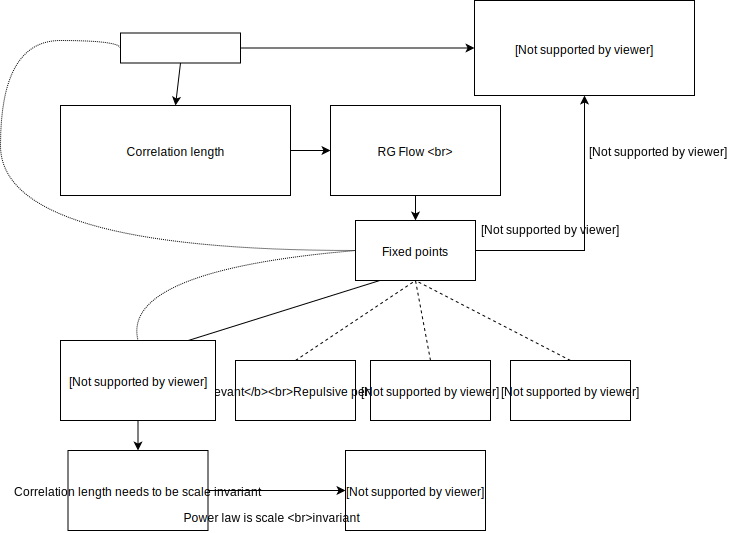
\includegraphics[scale=0.6]{figures/rg_flow_1.png}
	\caption{A schematic on how fixed points in RG flow mean different behaviours for temperatures}
\end{figure}

\subsection{A Second Look at Universality} 
We can understand the phenomena of universality 
much better now using the language of renormalisation. 
Let's begin by starting at one point in theory space, for example 
in the above case where $ \zeta = 1 $. 
We then start flowing to larger and larger $ \zeta $. 
Where can we land? 
We can't have cycles in theory space! We may be able to have 
shapes in theory space. 
Check out the C-theorem for more information about this. 
\begin{enumerate}
	\item We could have that our couplings like $ \mu^ 2 ( \zeta ) $. or $ g ( \zeta) `$, 
		could flow in some direction off to infinity. 
	\item More interestingly, we could have the coupling constants 
		converging towards a fixed point. At a fixed point, 
		the theory doesn't change with scale which implies that our correlation 
		length  $ \xi $ needs to be $ \xi = 0 $ or  $ \xi = \infty$, 
		since $ \xi $ depends on scale. 
\end{enumerate}

\subsubsection{The Ising model} 
Let's think about the case when $ T > T_c$, with $ 
T \to \infty$. We expect that at this temperature, 
spins change so rapidly that we don't expect the things to 
be correlated. Hence, we have that $ \xi \to 0$. 

On the other hand, when we're in the cold regime
with  $ T < T_ c $, and that  $ T \to 0 $, we also 
have that nothing happens so our correlation length 
$ \xi \to 0 $. 

Our most interesting case is when  $ T = T_c $, 
In this case, we have that  $ \xi \to \infty$, 
and we have fluctuations on every possible length scale. 
Colloquially, this looks like a fractal. 

\subsection{Classifying fixed points} 
Suppose we have a set of coupling constants in theory space. 
We can classify deformations in theory 
space based on how the flow changes towards fixed points. 

\begin{figure}[h]
	\centering
	\includegraphics[width=0.8\linewidth]{figures/deformations.png}
	\caption{Classifying deformations in theory space}%
	\label{fig:deformations}
\end{figure}


\subsection{Scaling}
Since all scales are washed away in the fixed point, 
we have that our correlation, which is a function of length, 
can only depend on this length scale. So, we must have that 
our correlation function must take the form of a power law. 
\[
	\left< \phi ( \vec{x} ) \phi ( 0 )  \right> = \frac{1}{ r ^{ d - 2 + \eta }}
\] In units of inverse length, we have that 
$ [ x ]  = - 1$,  $ \left[ \frac{\partial }{\partial x }   \right]  = 1 $. 
Since our free energy needs to be dimensionless, 
ie that $ [ F [ \phi ] ]  = 0 $, we have that our dimensions 
of our scalar field satisfies \[
	[ \phi ( \vec{x} ) ] = \frac{d -2  }{ 2 } \implies \eta = 0 
\] Assuming that under the scaling $ \vec{x} \to \frac{\vec{x} }{ \zeta}$, 
that our scalar field $ \phi ( \vec{x} ) \to \zeta ^{ \Delta_{ \phi } } \phi ( \vec{x} ) $, 
substituting this into our power law relation gives that 
\[
 \Delta_\phi = \frac{d -2 + \eta }{ 2 } 
\]  where we have that the $ \frac{d - 2 }{ 2 } $ is referred to 
as our engineering dimension, where are our extraneous factor 
of $ \frac{\eta }{ 2 } $ is referred to as our anomolous dimension. 
There's a difference here. However, we can reconcile this by 
setting 
\[
	\left< \phi ( \vec{x} ) \phi  (0 )  \right>  = \frac{a ^ \mu }{ r ^{ d - 2 + \eta }}
\] 
\subsection{Relation to critical exponents} 
Recall that our correlation length 
was derived as a function of our critical temperature 
\[
 \xi \sim t ^{  - `v }
\] However, since $ \xi $ is a length scale, this 
means it has scaling coefficient $ \Delta_\xi = - 1$. 
Assuming that our temperature scales like 
 \[
 t \to \xi^{ \Delta_t } t
\] we have that $ \Delta_t = \frac{1}{`v }$. 
Now consider the free energy without a magnetic field. 
At leading order, we have that 
\[
	F_{ \text{thermo } } ( t)  = \int d^ d x f( t) \implies f( t)  \sim t ^{ d \nu }
\] From this we can read off variables of interest. 
We have that 
\[
 c = \frac{\partial ^ 2 f }{\partial  t ^ 2 }  \sim t ^{ d \nu - 2 } \sim t ^{ - \alpha }
\]

So in summary, we have the following 
critical exponents, 
\begin{align*}
	c &=  \frac{\partial  ^ 2 f }{\partial   t^ 2 } \sim t ^{ - \alpha } \implies \alpha = 2 - d \nu  \\
	\phi  & \sim t ^ \beta \implies \beta = \left(  \frac{ d - 2 + \eta }{2} \right) \nu    \\
	\chi & \sim t ^{ - \gamma } \implies \gamma = \nu ( 2 - \eta ) \\
	\phi & \sim B ^{ \frac{1}{ \delta } } \implies \delta = \frac{ d + 2 - \eta }{ d - 2 + \eta }
\end{align*}

This is great because we've reduced the 
number of parameters which we need to measure! We have 
four observables but only need to determine $ \eta $ and $ \nu $. 
Hence, 
our theory is useful!

\begin{table}[htpb]
	\centering
	\caption{caption}
	\label{tab:label}
	\begin{tabular}{c | c c c c c c }
		MF & $ \frac{ 4 - d }{ 2 } $ & 1 & 3 & 0 & $\frac{1}{2 } $ \\
		$ d =  2 $ & 0  & $ \frac{1}{8 } $  & $ \frac{7}{4 } $ &  $ 15 $ & $\frac{1}{4 } $ & 1 \\
		$ d = 3 $ & 0.11 & 0.33 & 1.24 & 4.79 & 0.04 & 0.63 \\ 
	\end{tabular}
\end{table}


\subsection{Relevant, Irrelevant or Marginal?} 
Consider our free energy given by our usual expression 
\[
	F [ \phi ] \sim \int d^ d x \left\{  + \dots + g_{ \mathcal{ O } } \mathcal{ O } ( \vec{x} ) + \dots  \right\}  
\]  We could have a special case 
where our operator $ \mathcal{ O } $ scales \textbf{nicely}
with our renormalisation group flow. This is not usually, 
the case and its hard to find operators which behave in this way, 
but bear with me for a moment and let's assume that this is the case. 
\[
	\mathcal{ O } ( \vec{x} ) \to \mathcal{ O } ' ( \vec{x} ' ) = \zeta^{ \Delta_{ \mathcal{ O } } } \mathcal{ O } ( \vec{x} ) 
\] So, we can 
think of $\mathcal{ O } $ as an eigen-operator 
of our RG flow process. Now, in the above expression 
we have coupled $ g_{ \mathcal{ O } } $ as the coupling constant. 
Due to the dimensionless constraint of our free energy, 
we have that 
\[
 \Delta g_{ \mathcal{ O } } = d - \Delta _{ \mathcal{ O } }
\] This implies that $ g_{ \mathcal{ O } }$ goes 
off to infinity, zero, or stays where it is depending
on the sign on $ \Delta g ^{ \mathcal{ 0 }}$. 

\begin{enumerate}
	\item $ \Delta_{ \mathcal{ O } } < d \implies $ Relevant 
	\item $ \Delta_{ \mathcal{ O } } > d  \implies $ Irrelevant
	\item $ \Delta_{ \mathcal{ O } }  = d \implies $ Marginal 
\end{enumerate}


\subsection{The Gaussian fixed point} 
Let's consider what happens 
when we have our usual free energy to quadratic order. 
Recall that we have the fourier expansion 
\[
	F _ 0 [ \phi ] = \int d^ d x \left[  \frac{1}{2 } ( \nabla \phi ) ^ 2 + \frac{1}{2 } \mu _ 0 ^ 2 \phi ^ 2 \right] = \int_ 0 ^ \Lambda \frac{ d^ d k }{ ( 2 \pi ) ^ d } \frac{1}{2 } \left(  k ^ 2 + \mu_ 0 ^ 2   \right)  \phi 
	_{ \vec{k} } \phi _{ - \vec{k}}
\] The useful thing about having 
a quadratic free energy like this 
is that this separates into low and high 
fourier modes with 
\[
	F _ 0 [ \phi ] = F_0 [ \phi ^ - ] + F _ 0 [ \phi ^ + ] 
\] This means that when we write out 
our effective free energy, we get that 
\begin{align*}
	e ^{  - F ' [ \phi ^ - ] } &= \left[  \int \mathcal{ D } \phi ^ + 
	e ^{  - F _ 0 [ \phi ^ +  ] }\right] e^{  - F_0 [ \phi ^ -  ] }    \\
				   &=  \mathcal{ N } e ^{  - F_ 0 [ \phi ^ - ] } \\
\end{align*}
After our rescaling procedure, 
we have that under our RG flow our 
coupling parameter scales like 
\[
 \mu ^ 2 ( \zeta ) = \zeta ^ 2 \mu ^ 2 _ 0 
\] Once we have this, we can find 
our fixed points which satisfy the relation 
$ \frac{ d \mu ^ 2  }{ \zeta} =0  $. Hence, we 
have that 
\[
 \mu ^ 2 = \infty, \quad \mu ^ 2 = 0  
\] Our point $ \mu ^ 2  = 0 $ is called our Gaussian 
fixed point. Right now, these
points are uninteresting!

\subsubsection{Around the fixed point} 
Let's generalise this further by expanding 
in higher orders of $ \phi $. 
We expand our free energy in a power series as
 \[
	 F [ \phi ]  = \int d ^ d x \left[ \frac{1}{2 } ( \nabla \phi ) ^ 2 + 
	 \frac{1}{2 } \mu ^ 2 _ 0 \phi ^ 2 + \sum_{ n = 4 } g_{ 0 , n } \phi ^ n \right]  
\]  Having these
extra terms mean that when we decompose our 
fourier modes into low frequency and 
high frequency modes, we have that 
the coupling constants shift. We thus have that 
\[
 g _{ 0 , n } \to g_{ n } ' = g _{ 0 , n } + \delta g _{ n }
\] We're in good shape to now 
perform RG flow on this free energy. 
Ignoring the shift we did above and scaling naively, 
we have that, 'input scaled function here
\[
 F ' [ \phi ' ] 
\] Insert graph on RG flow here.  
For our coupling constants, we 
then see that our flow induces a scaling on 
$ g_n $ via 
\[
 g _ n ( \zeta ) = \zeta ^{ d - n \Delta \phi } g_{ 0 , n }
\] This means that we can classify 
our deformations around fixed points depending on 
our dimension. So, we have that 
\begin{enumerate}
	\item $ d > 4 , \phi ^ 4 $ irrelevant 
	\item $ d < 4 , \phi ^ 4 $ Relevant 
	\item $ d  = 4, \phi ^ 4 $ Marginal 
\end{enumerate} 

\subsubsection{$ \mathbb{ Z} _ 2 $ Symmetry breaking } 
Typically, we have that RG flow doesn't break our 
symmetries. This symmetry is respected by momentum, 
so in momentum space symmetry is also preserved. This means 
that every term in our decomposition 
\[
 F_ 0 [ \phi ] = F_ 0 [ \phi ^ - ]  + F_0 [ \phi ^ + ] + F_I [ \phi ^ - , \phi ^ + ] 
\] At low temperature, 
our background magnetic field, becomes important. 
We need to have an RG way of visualising what's going on. 


\pagebreak 
\section{Example Sheet 1} 
\subsection{Question 1}
In this question, we're examining the partition function of a one dimensional, periodic $N$ atom lattice in the Ising model. 
Summing over all possible states $s_i = \pm 1$, with the boundary condition that $s_0 = s_N$, it's easy to see that the partition function takes the form 
\[ 
	Z = \sum_{s_1 = \pm 1} \dots \sum_{s_N = \pm 1} \prod_{i} \exp\left( \beta J s_i s_{i + 1} + \beta B (s_i + s_{i + 1}) \right). 
\]
Note that we've transferred the inner sum for our expression of $E$ into the outer product of exponentials to make this object easier to deal with. 

Given that the transfer matrix is 
\[ 
	T= \begin{pmatrix}
		e^{\beta J  - \beta B} & e^{ - \beta J} \\
		e^{ - \beta J} & e^{\beta J + \beta B}. 
	\end{pmatrix}
\]
we can index this matrix in a slightly different way which reflects spins. We index the elements in the array with ${\pm 1}$ instead of perhaps what we're used to with $\{ 0, 1\} $. Using the indices $s_i, s_{i + 1}$, we can write that 
\[ 
	T_{s_i, s_{i + 1}} = \exp \left (\beta s_{i} s_{i + 1} + \frac{\beta B}{2} (s_i + s_{i + 1}) \right) 
 \] 
 If we're trying to find out what $T^N$ is then in standard index notation, 
 \[ 
 	\left(  T^N \right)_{s_{1}, s_{N + 1}}= T_{s_1, s_2} T_{s_2, s_{3}} \dots T_{s_N, s_{N + 1}}
 \] 
 where we sum implicitly over pairs of identical indices. 
 Due to our periodicity condition, we have that $s_1= s_{N + 1}$, and since we're taking the trace we have 
 \[ 
 	Tr (T^N) = \left( T^N \right)_{s_1, s_1} = \sum_{s_1 = \pm 1} T_{s_1, s_2} T_{s_2, s_{3}} \dots T_{s_N, s_{1}}
 \] 
where we've kept the sum over $s_1$ explicit here. Making the sum over the rest of the terms explicit, and substituting in our expressions, for $T_{s_i, s_{i + 1}}$, gives the required result. 

Our characteristic equation for $ T $ is 
 \[
	 0 = ( e^{ \beta J - \beta B } - \lambda )( e^{\beta J + \beta B } - \lambda ) - e^{  - 2 \beta J }
\] Expanding out, we have the equation
\[
	0 = \lambda^ 2 - \lambda e^{ \beta J } ( e^{ \beta B } + e ^{ - \beta B } ) + e^{ 2\beta J }  - e^{  - 2 \beta J }
\] Using cosh and sinh expresions, and the quadratic formula, this is 
\[
	0 = \lambda^ 2 - 2 \lambda \cosh ( \beta B ) + 2 \sinh ( \beta B ) \implies \lambda_\pm = e^{ \beta J }\cosh ( \beta B ) \pm \sqrt{ e ^{ 2 B J } \cosh^ 2 ( \beta B ) - 2 \sinh ( \beta B ) } 
\] Now note that, if $ \lambda  $ is an eigenvalue of $ A$, then  $ \lambda^ n $ is an 
eigenvalue of  $ A^ n $, since repeated application of  $A $ on an
eigenvector pulls out  $n $ factors of $ \lambda $. 

Since the matrix $ T ^ n $ is two dimensional, it has at most 2 eigenvectors. 
We know that, for the previous reason, that $ \lambda_+ ^ n $ and  $ \lambda_-^ n $ 
are eigenvalues of  $ T ^n $, so they're all of the eigenvalues. 
Since the trace of a matrix is the sum of its eigenvalues, 
 \[
	 Tr ( T ^ N ) = \lambda_+^ N + \lambda_- ^ N  = \lambda_+^N ( 1 + (\frac{\lambda_-}{\lambda_+ })^ N) \to \lambda_+^N , \quad N \to \infty 
\] The term in the bracket goes to 1 since in this case $  \mid \lambda_-  \mid $ is less than $  \mid  \lambda_+  \mid $. 
Asymptotically as $ N \to \infty$, we have that 
\[
 m  = \frac{1}{N \beta } \frac{\partial \log Z}{\partial B } \sim \frac{1}{N \beta } N \frac{\partial \log \lambda_+ }{\partial B } 
\] But we have that 
\[
	\frac{\partial  \lambda_+ }{\partial B }  = e^{ B J }\beta \sinh ( \beta B ) + \frac{\beta e^{ 2 \beta J } \cosh ( \beta B ) \sinh ( \beta B ) }{\sqrt{ e ^{ 2 B J } \cosh ^ 2 ( \beta B ) - 2 \sinh ( \beta B ) } }
\] But this is just $0 $ at $ B = 0 $ since we can factor out $ \sinh ( \beta B ) $. 
Hence, our magnetisation at equilibrium is  $ 0 $ regardless of temperature. 
So our free energy is fixed at $ f( 0 )$, which is constant and therefore continuous. So, 
we have no phase transitions based on temperature. 

\pagebreak 
\subsection{Question 2}
Our energy expression for the Ising model is
\[
	E = - B \sum_i s_i - J\sum_{\langle i j \rangle} s_i s_j
\]
where in the last term we sum across neighbouring pairs of atoms on the lattice. Writing out 
\[ 
	s_i  = (s_i - m) + s_i
\]
where we now assume $(s_i - m)$ is small, we have that 
\begin{align*}
	s_i s_j &= \left( s_i - m + m \right) \left( s_j - m + m \right) \\
		   &= (s_i -m)(s_j - m) + m^2  + m (s_ j - m  + s_i  - m ) \\
		   &\approx m (s_i + s_j) - m^2. 
\end{align*}
Thus we have 
\begin{align*}
	\sum_{\langle ij \rangle} s_i s_j = \sum_{\langle i j \rangle} \left( m (s_i + s_j) - m^2 \right)  = q m \sum_i {s_i}- \frac{m^2 q N }{2}
\end{align*}
Hence we have that 
\[ 
	E = - (B + J qm )\sum_i s_i  + \frac{J q m N^2}{2}
\]
Since we've gotten rid of our interaction term and can factor this expression out in $s_i$, all we have to do is calculate $Z$ for a single particle only, then take this to the power $N$. This is because the partition function is factorable. For a single particle, we sum over both spin configurations
\[ 
	Z_i = e^{ -\beta J q m^2 / 2} \left( e^ { - \beta B_{\text{eff}}} + e^{\beta B_{\text{eff}}} \right) = 2 e^{ -\beta J q m^2 / 2} \cosh (\beta B_{\text{eff}}), \quad B_{\text{eff}} = B + J q m
\]
For the whole system we get that 
\[ 
	Z = e^{ -\beta J N q m^2 / 2}2^N \cosh^N  (\beta B_{\text{eff}})
\]
Using our expression that the partition function is well approximated by 
\[ 
	Z \approx e^{- \beta N f(m_{\min})}
\]
we equate this to our expression above and find that our free energy as a function of magnetisation is 
\[ 
	f(m) = \frac{1}{2}J q m^2 + \frac{1}{\beta} \log{2 \cosh ( {\beta J qm + \beta B }) }
\]
Minimising this function gives us the self-consistency equation 
\[ 
	\frac{\partial f }{\partial m } = 0 \implies m = \tanh (\beta(J qm + B)). 
\]

\pagebreak 
\subsection{Question 3}
Setting $m = \frac{1}{N} \sum_i s_i$, our expression for $E$ is 
\[ 
	E =  - B \sum_i s_i  - \frac{J}{2N} \left( \sum_i s_ i \right) \left( \sum_j s_j \right)  = - BNm - \frac{J q Nm^2}{2}
\]
If the extra divisor of $N$ wasn't there, we'd have a factor of $N^2$ in our second term, which means that our expression for our free energy $f(m)$ would depend on N. 

As before, we apply mean field theory and remove small terms quadratic in $s_i - m$ to find that 
\[ 
	E = - B \sum_i s_i +  \frac{JNm^2}{2} - J m \sum_i s_i  = - (B + Jm ) \sum_i s_i + \frac{JNm^2}{2}. 
\] 
so our partition function is reduced to the partition function for the neighbour Ising model with $q = 1$: 
\[
	Z =  e^{ - \beta J N m^2 / 2}2^N \cosh^N(\beta(J m + B)). 
\]
We verify the identity in the question by completing the square in the exponent 
\begin{align*}
	\sqrt{\frac{N \beta J }{2 \pi}} \int_{ -\infty}^{\infty} e^{ - N \beta J x^2 / 2 + \alpha \beta J x } dx&= \sqrt{\frac{N \beta J }{2 \pi}} \int_{- \infty}^{\infty} e^{ - \frac{N \beta J }{2} ((x - \frac{\alpha}{N})^2 - \frac{\alpha^2}{N^2})}dx \\ 
		&= \sqrt{\frac{N \beta J }{2 \pi}} e^{\frac{\alpha^2 \beta J }{2 N }} \int_{ - \infty}^{\infty} e^{ -\frac{N \beta J }{2} (x - \frac{\alpha}{N})^2} \\
		&= e^{\frac{\alpha^2 \beta J }{2 N }}
\end{align*}



Our energy is of the form 
\[
	E = - B\sum_i s_i - \frac{J}{2N}\left( \sum_i s_i \right) \left( \sum_j s_j \right)  
\]
but to use mean field theory, we set 
\[
	\sum_i s_i = Nm \implies E = - BNm - \frac{JNm^2}{2} 
\]
so we have that for a given magnetisation $m$, 
\[
	e^{ - \beta E(m) } = \exp(\beta B Nm + \frac{\beta JNm^2}{2}) 
\]
From the previous identity, we have that setting $\alpha = 0$ gives us the identity 
\[
	1 = \sqrt{\frac{N \beta J}{2 \pi}} \int_{ - \infty}^{\infty} \, dx \exp( - N \beta J \frac{x^2}{2}) 
\]
We do a clever translation by the constant $m$ so that 
\[
	1 = \sqrt{\frac{N\beta J}{2 \pi}} \int_{-\infty}^\infty dx \, e^{ - N \beta J (x - m)^2 / 2}
\]
and once we translate this, we can multiply this expression by $e^{ - \beta E(m)}$
\[
	e^{ - \beta E(m)} = \int_{ - \infty}^\infty dx \, e^{ - N \beta J (x - m)^2  / 2}e^{\beta B N m}e^{\beta J N m^2 / 2}.
\]
which simplifies to 


\[
e^{ - \beta E(m)} = \sqrt{\frac{N \beta J}{2 \pi}} \int_{ - \infty}^{\infty} dx \, e^{ - \frac{N \beta J x^2}{2}}e^{ - \beta Nm(J x + b)}  
\]
We rewrite this in terms of our decoupled spin sums to get 
\[
e^{ - \beta E} = \sqrt{\frac{N \beta J }{2 \pi}} \int_{ - \infty}^\infty e^{ - N \beta J x^2 / 2}e^{ - \beta \left(  \sum_i s_i \right) (Jx + B)}
\]

Our partition function $Z$ comes from all possible configurations of our spins. 
\[	
Z = \sqrt{\frac{N \beta J}{2 \pi}} \int_{-\infty}^{\infty} dx \, e^{ - N \beta J x^2  / 2} \sum_{\{ s_i \}} e^{ - \beta \sum_i s_i (Jx +B)} 
\]
We can use the fact that we have a separable form here to factor out the sum over all possible spin configurations. 
\[	
\sum_{\{ s_i \}} e^{ - \beta \sum_i s_i (Jx + B) } = \prod_{i}\sum_{s_i = \pm 1} e^{ - \beta \sum_i s_i (Jx + B)} = (2 \cosh (Jx  +B))^N 
\]
Substituting this into out integral gives us the result that we want.
Items:
\begin{itemize}
\item Tried expanding the exponential representation of cosh binomially. 
\item Messing around with substitutions?
\end{itemize}

\pagebreak 
\subsection{Question 4}

\subsubsection*{Sketching out our functions} 
We're interested in the behaviour of the function 
\[ 
f(m) = \alpha_2 (T) m^2 + \alpha_4 m^4 + \alpha_6 m^6, \quad \alpha_4 < 0 
\] We first differentiate and see where roots exist. 
\[
f ' ( m ) = 2 m ( \alpha_2 + 2 \alpha_4 m^2 + 3 \alpha_6 m ^ 4 ) 
\] This implies that $ m = 0 $ is always a stationary point. 
We focus our attention to solving for roots of the quadratic factor. 
Without caring abotu signs for now, solving the equation as 
a quadratic in $ m^ 2 $ then square rooting gives 
\[
m = \pm \sqrt{  - \frac{\alpha_4 }{3 \alpha_6 } \pm  \frac{1}{ 3 \alpha_6 } \sqrt{ \alpha_4^2 - 3 \alpha_6 \alpha_2 }} 
\] Now, the number of real solutions depends on signs. 
This equation has no real solutions when $ \alpha_2 > \frac{ \alpha_4 }{ 3 \alpha_6 }$. 
Thus, $ m = 0 $ is our only stationary point. Our function is 

\begin{figure}[h]
\centering
\begin{tikzpicture}[scale=0.7]
\begin{axis}[ 
xlabel=$m$,
ylabel={$f(m)$}, 
axis x line=center,
axis y line=center,
ticks=none, 
no markers, 
clip=false 
] 
\addplot { x^6 }; 
\end{axis}
\end{tikzpicture} 
\end{figure} 

After this, we have only two real solutions 
in the case when  $ \alpha_2 < 0 $, is this implies that only 
$ \frac{ - \alpha_4 }{3 \alpha_6 } + \frac{1 }{ 3 \alpha_6 }\sqrt{ \alpha_4^2  - 3 \alpha_6 \alpha_2 } $ 
is positive in the square root. 
This means our only stationary points are at 0 and two other places. 
we know it's this shape since around zero, $m^2 $ term dominates and we should have a negative 
quadratic. 

\begin{figure}[h]
\centering
\begin{tikzpicture}[scale=0.8]
\begin{axis}[ 
samples=150, 
xlabel=$m$,
ylabel={$f(m)$}, 
axis x line=center,
axis y line=center,
ticks=none, 
no markers, 
restrict x to domain*=-2:2,
restrict y to domain*=-3:5,
xmin=-2,
xmax=2,
ymin=-3, 
ymax=5,
clip=false 
] 
\addplot {x^6 -   x^4  -  x^2 }; 
\end{axis}
\end{tikzpicture} 
\caption{This our metastable state disappears when $\alpha_2 ( T ) $ is below 0!}
\end{figure}

In our final case we have that for $ 0 < \alpha_2 < \frac{\alpha_4^2 }{3 \alpha_6 }$ 
we have five stationary points including zero. 
The only possible configurations for stationary points is that 
$ m_0  = 0, m_\pm  = \pm \sqrt{  - \frac{\alpha_4}{3\alpha_6 } + \frac{1}{3 \alpha_6 } \sqrt{ \alpha_4^2 - 3 \alpha_6 \alpha_2 } } $ 
must be minima, and the other points are maxima. 

Our condition for $ m_\pm$ to be \textbf{global} minima (not metastable states) 
is that we must have that $ f ( m_\pm) $ must be smaller than $ f (m_0 ) = 0 $. 
Algebra shows that 
\begin{align*}
m_\pm^2 & =  - \frac{\alpha_4}{\alpha_6 } + \frac{1}{ 3 \alpha_6 } \sqrt{ \alpha_4 ^ 2 - 3 \alpha_6 \alpha_2 } \\
m_\pm^ 4 & = \frac{1}{ 9 \alpha_6 ^ 2 } ( 2 \alpha_4 ^ 2 - 3 \alpha_6 \alpha_2  - 2 \alpha_4 \sqrt{ \alpha_4^2 - 3 \alpha_6 \alpha_2 } 
\end{align*}

So substituting this into $ f ( m ) $ gives 
 \begin{align*}
	 f ( m_\pm ) &= m_\pm^2 ( \alpha_2 + \alpha_4 \left(  - \frac{\alpha_4}{3 \alpha_6 } + \frac{1}{3\alpha_6 } \sqrt{ \alpha_4^  2 - 3 \alpha_6 \alpha_2}  \right) \\
		     & +  \frac{\alpha_6}{9 \alpha_6 ^ 2 } \left( 2 \alpha_4 ^ 2 - 3 \alpha_6 \alpha_2 - 2 \alpha_4 \sqrt{ \alpha_4 ^ 2  - 3 \alpha_6 \alpha_2 }  \right)) \\
		     &= m_\pm^2 ( \frac{ 2 \alpha_2 }{ 3 } - \frac{ \alpha_4^ 2 }{ 9 \alpha_6 } + \frac{\alpha_4 }{ 9 \alpha_6 } \sqrt{ \alpha_4  - 3 \alpha_6 \alpha_2} ) 
\end{align*}
Hence, we require that the term in the brackets is negative. 
If we multiply by $ 9 \alpha_6  > 0 $, our condition 
becomes that 
\begin{align*}
	6 \alpha_2 \alpha_6 - \alpha_4^ 2 + \alpha_4 \sqrt{ \alpha_4 ^ 2 - 3 \alpha_6 \alpha_2 }  & <  0  \\
	6 \alpha_2 \alpha_6- \alpha_4^ 2 <   - \alpha_4 \sqrt{ \alpha_4^  2 - 3 \alpha_2 \alpha_6 } 
\end{align*}
Squaring both sides, cancelling an $ \alpha_4 ^ 4 $ in the sum on each side,  and then cancelling 
$ \alpha_ 2 $ gives us the condition that 
 \[
  36 \alpha_2 \alpha_6 ^ 2 - 12 \alpha_4 ^ 2 \alpha_6 <  - 3 \alpha_4 ^ 2 \alpha 6 \implies \alpha_2 < \frac{ \alpha_4 ^ 2 }{4 \alpha_6 }
\] So, we get that our magnetisation jumps by $ m_\pm $ only when 
these points become a global minimum, at  $ \alpha_ 2  = \frac{\alpha_4 ^ 2 }{ 4 \alpha_6 }$ 

\begin{figure}[h]
	\centering
	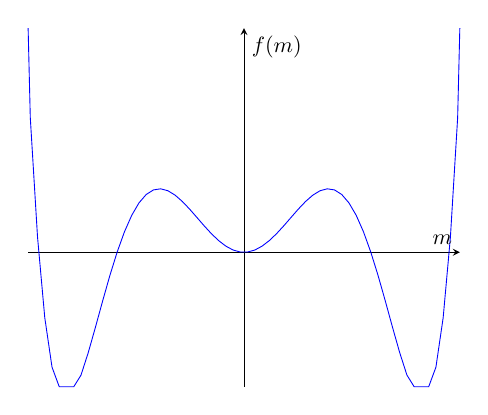
\begin{tikzpicture}[scale=0.8]
  \begin{axis}[ 
    samples=150, 
    xlabel=$m$,
    ylabel={$f(m)$}, 
    axis x line=center,
    axis y line=center,
    ticks=none, 
    no markers, 
    restrict x to domain*=-2:2,
    restrict y to domain*=-3:5,
    xmin=-2,
    xmax=2,
    ymin=-3, 
    ymax=5,
    clip=false 
  ] 
    \addplot {x^6 - 5 *  x^4 + 5 * x^2 }; 
  \end{axis}
\end{tikzpicture}
\quad 
	\begin{tikzpicture}[scale=0.8]
  \begin{axis}[ 
    samples=150, 
    xlabel=$m$,
    ylabel={$f(m)$}, 
    axis x line=center,
    axis y line=center,
    ticks=none, 
    no markers, 
    restrict x to domain*=-1.0:1.0,
    restrict y to domain*=-0.1:1.5,
    xmin=-1,
    xmax=1,
    ymin=-0.1, 
    ymax=1.5,
    clip=false 
  ] 
    \addplot {x^6 -  x^4 +0.3*  x^2 }; 
  \end{axis}
\end{tikzpicture}


 \caption{Left: when $ \frac{ \alpha_4^2}{ 4 \alpha_6} > \alpha_2 > 0$; we have a metastable state at $m = 0$. 
 On the right is what happens otherwise.}
\end{figure} 

Because of this jump, we have a phase transition. 

\subsubsection*{Showing a first order phase transition} 
For ease of notation let's denote the global minimum of $ f $
as  $ m_0 $ in either case. 
When $ \alpha_2 > \alpha_{ c } = \frac{ \alpha_4^ 2 }{4 \alpha_6 }$, we have $ f ( m _0 ) = 0$. 
Let's write our the energy in terms of $  m_0$ and differentiate with 
respect to the parameter $\alpha_2 $, denoted with an apostrophe. 
We have 
\begin{align*}
	f( m_0 ) &=  \alpha_2( T ) m_0^ 2 + \alpha_4 m_0 ^ 4 + \alpha_6 + m_0 ^ 6  \\
	f' ( m_ 0 ) & = 2 \alpha_2 m_0 m_0' + m_0^ 2 + 4\alpha_4 m_0 ^ 3 m_0' + 6 \alpha_6 m_0^ 5 m_0' \\
		    &=  m_0 ^ 2 + 2 m_0 m_0' (  \alpha_2 + 2 \alpha_4 m_0^ 2 + 3 \alpha_6 m_0 ^ 4 )  \\
		    &=  m_0 ^ 2  \\
\end{align*}
We took the last term to zero since $ m_0 $ solved this equation earlier. 
Now, if we take the limit as $ \alpha_2 \to \frac{ \alpha_4 ^ 2 }{4  \alpha_6 }$, 
it's easy to verify that 
\[
	m_0 =  - \frac{\alpha_4 }{3 \alpha_6 }+ \frac{1}{3 \alpha_6 }\sqrt{ \alpha_4^ 2 - 3 \alpha_2 \alpha_6 } \to  - \frac{1}{6 }\frac{\alpha_4 }{\alpha_6 }  
\] This is non zero. So, we have a discontinuity as we vary $ f( m_0 ) $ with respect to this parameter. 
\subsubsection*{Critical exponents} 
At $\alpha_4 = 0$, we have that 
\[ 
m \sim ( - \alpha_2)^{ \frac{ 1}{ 4} }  
\] 
The question is, how do we get a critical exponent from this with the condition that $\alpha(T_c)$  = 0? Critical exponents occur when $T \rightarrow T_c$, which means that $( T  - T_c)^2$ is small. We can Taylor expand $\alpha_2$ around the critical temperature as
\[ 
\alpha_ 2( T ) = \alpha_2(T_c) + ( T - T_c ) \alpha_2'(T_c) + \frac{ ( T - T_c)^2}{ 2} \alpha_2''(T_c) + \dots \sim ( T  - T_c) \text{ at leading order }
\] 
Substituting this in the expression above, we then must have that 
\[ 
m \sim ( T_c - T )^{ \frac{1}{4} } 
\] which implies that our critical exponent $\beta = \frac{1}{ 4} $ Now, for heat capacity, assuming that $\alpha_2 = K(T  - T_c ) $ to leading order, we have that our free energy can be written as 
\[ 
f(m) = \frac{  K^{ \frac{3}{2} } }{ ( 3 \alpha_6 )^ \frac{ 1}{ 2}}(  T_c - T )^{ \frac{3}{2}} + \frac{1 }{ 3 \alpha_6 } (T_c  - T )^3 
\] Now we can calculate our critical exponent for heat capacity! Heat capacity per unit volume is defined as 
\[ 
c = \frac{1}{N } \beta^2 \frac{ \partial }{ \partial \beta^2 } \log Z  = \left(  T^2 \frac{ \partial^2 }{ \partial T^2 } + 2T \frac{ \partial }{ \partial T } \right) \frac{ 1}{ T} f(m)
\] However, recall that since we're eventually taking a limit as $T \rightarrow T_c$, we only need to find the leading order contribution of $(T_c - T)^k$ from our expression above. This is akin to just differentiating the $( T_c - T ) terms $, and not caring about anything else. So, differentiating the first term twice in our expression for $f(m)$ gives a leading order contribution of $(T_c  - T)^{ - \frac{ 1}{2} } $, so $\alpha  = \frac{ 1}{2} $. 

To calculate $\delta$, observe that at the critical point with $\alpha_2 = 0$, our free energy is given by 
\[ 
f(m ) =  -B m + \alpha_6 m^6 
\] Solving for $f'(m) = 0 \implies \delta = 5$.  

To calculate our magnetisation constant, we define our new free energy as 
\[
g ( m )   = - Bm + \alpha_2 m^ 2 + \alpha_6 m ^ 6 
\] Consider the case when $\alpha_2 < 0 $.  We want to find our new minimum point such that this function is minimised. 
We work perturbatively. The minimum point $ m_0  \neq 0 $ for our free energy 
without magnetic field satisfies 
\[
f ( m )  = \alpha_2 m ^ 2  +\alpha_6 m ^ 6 \implies 0  = f' ( m_0 ) =  2m_0 ( \alpha_2 + 3 \alpha_6 m_0 ^ 4 ) 
\] We have that 
\[
g '( m ) = - B + 2m ( \alpha_2 + 3 \alpha_6 m ^ 4 ) 
\] We assume that our minimum point for small $B $ takes the form 
\[
m' = m_0 + \epsilon 
\] So, to first order in $ \epsilon$, we have 
\begin{align*}
 0 = g' ( m' ) &=  - B + ( m_0 + \epsilon) ( \alpha_2 + 3 \alpha_6 ( m_0 + \epsilon) ^ 4 ) \\
	       & = - B + 2 ( m_0 + \epsilon)( \alpha_2 + 3 \alpha_6 m_0^ 4 + 12 \alpha_6 \epsilon m_0^ 4) \\
	       &= - B + 2 ( m_0 + \epsilon) ( 0 + 12 \alpha_6 \epsilon m_0^3 ) \\
	       &= - B + 24 m_0^4 \epsilon \alpha_6 
	  \end{align*}
So, we have that 
\[
	\epsilon = \frac{B }{ 24 m_0^4 \alpha_6 } = \frac{B }{ 24 \alpha_2 \alpha_6} \sim \frac{B }{ 24 ( T_c - T )  \alpha_6} 
\] Hence, our equilibrium magnetisation is
\[
 m ' = m_0 +  \frac{B }{ 24 ( T_c - T )  \alpha_6} \implies  \xi =\frac{\partial m' }{\partial B } \sim \frac{1}{T_c - T }
\] This was for the case $ \alpha_2 < 0 $, where $ m_0 \neq 0 $. 
Otherwise, when $\alpha_2 > 0 $, $m \sim 0 $ and thus we can truncate $ g $
 \[
 g ( m) = - B m + \alpha_2 m^2 \implies m' = \frac{B}{2 \alpha_2 } \implies \xi  \sim \frac{1}{ T - T_c}
\] where $ m' $ is simply found by differentiating $g $ and setting to 0. 
Thus, on either side of the phase, 
\[
\xi \sim \frac{1}{ | T - T_c | } \implies \gamma = 1
\] 


\pagebreak 
\subsection{Question 5} 
We're now mixing things up and are introducing a complex order parameter. Here, we're using the free energy associated with superfluid Helium. We have something that looks like an Ising type free energy, but has a different kind of symmetry. 
\[ 
	F(\psi) = \alpha_2 |\psi|^2 + \alpha_4 |\psi|^4 
\] We have $U ( 1) $ symmetry here since 
\[ 
	\psi \rightarrow e^{ i \theta} \psi, \quad \psi \in \mathbb{R} 
\] leaves our free energy invariant. Since the free energy just depends on the modulus of $\psi$, we don't have minimum points but minimum \text{contours}, and in this case it's a minimum circle when $\alpha_2 < 0$. This is because when $\alpha_2 < 0 $, 
\[ 
	\frac{ \partial f }{ \partial |\psi| } = 2 |\psi|( \alpha_2 + 2 \alpha_4 | \psi|^2 ) , \implies \text{ minimum at } |\psi|  = \sqrt{ \frac{  - \alpha_2}{ \alpha_4 }} 
\] This means that when we have an equilibrium state, $\psi$ \textbf{jumps} to a point on this minimum circle, to a well defined point with $ \psi = \sqrt{ \frac{  - \alpha_2 }{ \alpha_4 } } e^{i \theta^*} $, which breaks our $U ( 1)$ symmetry. 

\begin{figure}[h] 
\centering
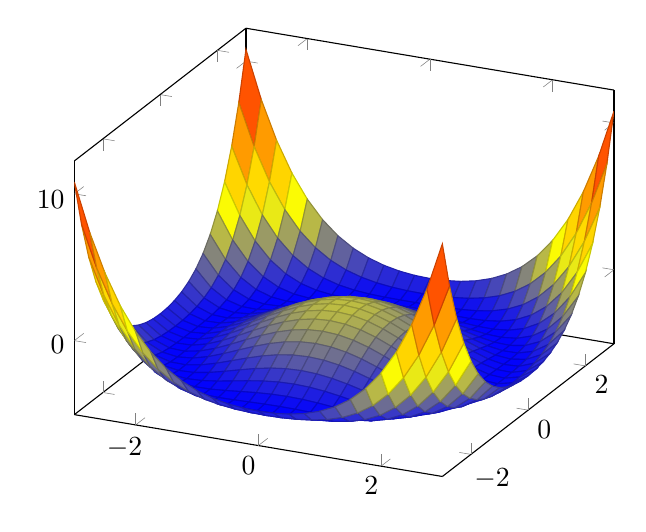
\begin{tikzpicture}
  \begin{axis}[domain=-3:3,y domain=-3:3]
    \addplot3[surf] { -1.2*( x^2 + y^2 ) + 0.1* (x^2 + y^2 )^2 };
  \end{axis}
\end{tikzpicture}
\caption{Our function where are x and y planes are identified with the real and imaginary parts of our complex parameter}
\end{figure} 

Now we work in the limit as $T \rightarrow T_c$, where since $\alpha_2( T_c) = 0$, we can Taylor expand this parameter as 
\[ 
	\alpha_2 \sim K ( T - T_c ) + \dots 
\] This implies that on our minimum contour we have that 
\[ 
	|\psi| \sim (T - T_c )^\frac{ 1 }{ 2 } \quad \beta = - 1 / 2, \text{ agrees with our Ising model} 
\] Furthermore, on our minimum contour we can calculate what our free energy is. Substituting for our value of $|\psi|$, we have that 
\[ 	
	f_{min} =  \begin{cases} 
		 - \frac{ \alpha_2^2 } { 2 \alpha_4 } \sim ( T - T_c)^2  & T < T_c \\
		 0 & T > T_c
		\end{cases} 
		\implies \log Z \sim \begin{cases} 
			\frac{ (T_c - T)^2 }{ T } & T < T_c \\
			0 
		\end{cases} 
\] But, this is exactly same as our limiting behaviour for our Ising model, where in our second chapter we showed that for the Ising model
\[ 
	\log Z = - \beta N f(m_{min} ) \implies \log Z =  - \beta N f(m_{min}) = \begin{cases} 
	0 & T > T_c \\
 N \frac{ 3}{ 4} \frac{ ( T - T_c)^2 }{ T}  & T < T_c 
\end{cases} 
\]  Thus, our critical exponent associated with heat capacity is $\alpha = 0$, exactly the same as the Ising model. This is kind of an example of universality! 

\pagebreak 
\subsection{Question 5} 

\subsubsection*{A rough physical model} 
In this question, we're exploring the phase transitions one has with an Ising model which takes our whole range of unit vectors as spins. We define an average magnetisation with the vector $\mathbf{m} $ with magnitude $m$, which obeys 
\[ 
	\mathbf{ m }  = \frac{ 1}{N} \sum_i \mathbf{s}_i
\] Substituting this into our energy, much like we did for the Ising model, we have that 
\begin{align*} 
	E &= - Jq \sum_{ \langle ij \rangle} \mathbf{s}_i \cdot \mathbf{s}_j + g \sum_i \left( ( s_z )^2_i - \frac{ 1}{2} ( (s_x)^2_i + ( s_y)^2_i )  \right) \\
	& \sim - JqN^2m^2 + N^2  g \left( m_z^2 - \frac{1}{2} ( m_y^2 + m_x^2 ) \right) 
\end{align*} 
Heuristically, and without much thought, we can identify the form of this model to the free energy that we get with the Ising model. Our best guess is that 
\[ 
	f(m, g, T) = \alpha_2 (  - 2g, T ) m_z^2  + \alpha_2( g, T) (m_x^2 + m_y^2 ) + \alpha_4 m^4 + \dots 
\] 
We've put in a factor of $ - 2$ in the first coefficient to account for the different proportions that each component has. Now, at first glance we have that (assuming the temperature is not too high such that magnetisations become disordered); 
\begin{itemize} 
	\item For $g > 0$ it is energetically favourable for magnetisations to lie in the $( x, y)$ plane due to the negative $ ( m_y^2 + m_x^2 )$ term, and hence our set of states which minimise free energy is a contour in the plane is the limit as $g \rightarrow \infty$. This is completely analogous to the $XY$ ordered case that we encountered in the previous question, where we can identify $m_x, m_y$ with a complex order parameter 
	\[ 
		\psi = m_x + i m_y 
	\] In the previous question, we showed that in the XY model, heat capacity is discontinuous as a result of differentiation twice with respect to $\beta$. This means that we have a second order phase transition when we increase the temperature. 
	\item For $g  < 0$ it is energetically favourable for our spins to lie in the $z$ direction, and, ignoring magnetisations $m_x, m_y$, we have that our energy is of the form 
	\[ E \sim   N^2 ( g - Jq)m_z^2, \text{ akin to the Ising model but without a magnetic field } \] Thus, we have an Ising type order here, and thus we again have a second order phase transition when we increase the temperature. 
\end{itemize} 
We can explicitly calculate that our transition is a first order phase transition when we move from $g< 0$ to $g > 0$. In the regime with $g > 0$, ignoring $m_z$, we have that 
\[ 
	f(m, g, T) = \alpha_2( g, T) (m_x^2 + m_y^2) + \alpha_4 ( m_x^2 + m_y^2)^2 \implies m_{min} = \sqrt{ \frac{  - \alpha_2 ( g, T ) }{ 2 \alpha_4 } } 
\] Thus, our free energy with $g > 0 $ is given by 
\[ 
	f_{min} = \begin{cases}  - \frac{ \alpha_2^2 ( g, T ) }{ 4 \alpha_4 }  & g > 0 \\
	         - \frac{ \alpha_2^2 (  - 2 g, T ) }{ 4 \alpha_4 } & g < 0 
	         \end{cases}
\] To get the order of our phase transition, we differentiate the free energy with respect to the parameter $g$, so that 
\[ 
	\frac{ df}{ dg} = \begin{cases} 
		 - 2 \frac{ \alpha_2 (g, T ) \alpha_2' ( g, T ) }{ 4 \alpha_4 } & g > 0 \\
		  4 \frac{ \alpha_2 (g, T ) \alpha_2' ( -2g, T ) }{ 4 \alpha_4 } & g < 0 \\
\end{cases} 
\] 
Now, as $g \rightarrow 0$, this is discontinuous in general since we have a factor of $2$ multiplier in the $g < 0$ regime. 

\pagebreak 

\subsection{Question 7} 
We substitute our expression of $\psi = A_k e^{ - ikx} $ into our expression for free energy. This gives us the free energy integral 
\[ 
	F = \int d^3 x\, \,  \alpha_2 (T) |A_k|^2 + \alpha_4 |A_k|^4  - k^2 \gamma |A_k|^2 + \kappa k^4 |A_k|^2
\] Now, assuming our mode satisfies $\frac{ dA_k }{ dk }  = 0$, differentiating the integrand with respect to $k$ gives us a minimum value of $ k$ at 
\[ 
	k_0^2 = \frac{ \gamma}{ 2 \kappa } 
\] Substituting this back into our integral gives us a thermodynamic free energy of 
\[ 
	F  = \int dx \left( \alpha_2( T) - \frac{ \gamma^2}{ 4 \kappa } \right) |A_k|^2 + \alpha_4 |A_k|^4 
\]  
Now, we can view $F$ as a function of the complex parameter $|A_k|$. We find that if $\alpha_2 > \frac{ \gamma^ 2}{ 4 \kappa } $, then our to minimise our free energy we have to force $|A_k| = 0 $ Hence $F = 0$ and our field configuration $\psi = 0$. However, in the case where $\alpha_2 <  \frac{ \gamma^ 2}{ 4 \kappa} $, we have that our parameter $|A_k|$ is minimised at \[ 
|A_k | =  \pm \sqrt { \frac{ \frac{ \gamma^ 2}{ 4 \kappa} - \alpha_2 ( T ) }{ 2 \alpha_4 }  }  , \quad \psi \neq 0 
\] But this means precisely that $\psi \sim e^{ ikx} $ is spatially modulated.



\end{document}
